% **************************************************
% Document Class Definition
% **************************************************
\documentclass[%
    paper=A4,               % paper size --> A4 is default in Germany
    twoside=true,           % onesite or twoside printing
    openright,              % doublepage cleaning ends up right side
    parskip=half,           % spacing value / method for paragraphs
    chapterprefix=true,     % prefix for chapter marks
    12pt,                   % font size
    headings=normal,        % size of headings
    bibliography=totoc,     % include bib in toc
    listof=totoc,           % include listof entries in toc
    titlepage=on,           % own page for each title page
    captions=tableabove,    % display table captions above the float env
    chapterprefix=false,    % do not display a prefix for chapters
    appendixprefix=false,    % but display a prefix for appendix chapter
    draft=false,            % value for draft version
]{scrreprt}%


% **************************************************
% Setup  thesis document in this file !
% **************************************************
% !TEX root = my-thesis.tex


% **************************************************
% Files' Character Encoding
% **************************************************
\PassOptionsToPackage{utf8}{inputenc}
\usepackage{inputenc}



% **************************************************
% Information and Commands for Reuse
% **************************************************
\newcommand{\thesisTitle}{Tesis Nombre}
\newcommand{\thesisName}{Marco Antonio Aguilar Gallardo}
\newcommand{\thesisSubject}{Innovación educativa para el desarrollo de México}
\newcommand{\thesisDate}{\today}
\newcommand{\thesisVersion}{Versión 3.0}

\newcommand{\thesisFirstReviewer}{Antonio Flores Moreno}
\newcommand{\thesisFirstReviewerUniversity}{\protect{Asesor Tecnico}}
\newcommand{\thesisFirstReviewerDepartment}{Maestro en ciencias}

\newcommand{\thesisSecondReviewer}{Edith Hernandez Hernandez}
\newcommand{\thesisSecondReviewerUniversity}{\protect{Asesor de estilo}}
\newcommand{\thesisSecondReviewerDepartment}{Profesora}

\newcommand{\thesisFirstSupervisor}{Antonio Flores Moreno}
\newcommand{\thesisSecondSupervisor}{Maria del Carmen}

\newcommand{\thesisUniversity}{\protect{Proyecto de titulación}}
\newcommand{\thesisUniversityDepartment}{Departamento de Ingeniería}
\newcommand{\thesisUniversityInstitute}{Universidad Aeronáutica en Querétaro}
\newcommand{\thesisUniversityGroup}{Ingeniería en Electrónica y Control de Sistemas de Aeronaves}
\newcommand{\thesisUniversityCity}{Querétaro}
\newcommand{\thesisUniversityStreetAddress}{Carretera Estatal 200 Querétaro – Tequisquiapan No. 22154 }
\newcommand{\thesisUniversityPostalCode}{76278}


% **************************************************
% Debug LaTeX Information
% **************************************************
%\listfiles


% **************************************************
% Load and Configure Packages
% **************************************************
\usepackage[spanish]{babel} % babel system, adjust the language of the content
\PassOptionsToPackage{% setup clean thesis style
    figuresep=colon,%
    hangfigurecaption=false,%
    hangsection=true,%
    hangsubsection=true,%
    sansserif=false,%
    configurelistings=true,%
    colorize=full,%
    colortheme=bluemagenta,%
    configurebiblatex=true,%
    bibsys=biber,%
    bibfile=Referencias,%
    bibstyle=alphabetic,%
    bibsorting=nty,%
}{cleanthesis}
\usepackage{cleanthesis}

\hypersetup{% setup the hyperref-package options
    pdftitle={\thesisTitle},    %   - title (PDF meta)
    pdfsubject={\thesisSubject},%   - subject (PDF meta)
    pdfauthor={\thesisName},    %   - author (PDF meta)
    plainpages=false,           %   -
    colorlinks=false,           %   - colorize links?
    pdfborder={0 0 0},          %   -
    breaklinks=true,            %   - allow line break inside links
    bookmarksnumbered=true,     %
    bookmarksopen=true          %
}

% **************************************************
% Other Packages
% **************************************************
\usepackage{scrhack}
\usepackage{graphicx,lipsum,afterpage,caption}
\usepackage{biblatex}
\usepackage[nottoc]{tocbibind}
\usepackage{amssymb, amsmath, amsbsy, amsfonts}    % ECUACIONES Y SÍMBOLOS MATEMÁTICOS
\usepackage{mathrsfs}                    % para formato de letra en ecuaciones
\usepackage{amsthm}     %Libreria para agregar teoremas
\usepackage{algpseudocode}
\usepackage{algorithm}
\usepackage{listings}
\usepackage{color}

% generar los cuadros de color---------------------------------------------------
\usepackage{tcolorbox}
\tcbuselibrary{listingsutf8} % o listings o minted
% Cuadro numerado para ejemplos
\newtcolorbox[auto counter, number within=section]{example}[2][]
{colback=green!5!white,colframe=green!75!black,
fonttitle=\bfseries, title=Función~\thetcbcounter: #2,#1}
% generar los cuadros de color---------------------------------------------------


\theoremstyle{definition}
\newtheorem{definition}{Definición}[section]
 
\lstset{ frame=Ltb,
framerule=0pt,
aboveskip=0.5cm,
framextopmargin=3pt,
framexbottommargin=3pt,
framexleftmargin=0.4cm,
framesep=0pt,
rulesep=.4pt,
backgroundcolor=\color{gray97},
rulesepcolor=\color{black},
%
stringstyle=\ttfamily,
showstringspaces = false,
basicstyle=\small\ttfamily,
commentstyle=\color{gray45},
keywordstyle=\bfseries,
%
numbers=left,
numbersep=15pt,
numberstyle=\tiny,
numberfirstline = false,
breaklines=true,
}

% minimizar fragmentado de listados
\lstnewenvironment{listing}[1][]
{\lstset{#1}\pagebreak[0]}{\pagebreak[0]}

\lstdefinestyle{consola}
{basicstyle=\scriptsize\bf\ttfamily,
backgroundcolor=\color{gray75},
}

\lstdefinestyle{C++}
{language=C++,
}

\definecolor{gray97}{gray}{.97}
\definecolor{gray75}{gray}{.75}
\definecolor{gray45}{gray}{.45}


% **************************************************
% Document CONTENT
% **************************************************
\bibliography{Referencias}              %Archivo .bib
\begin{document}

% uncomment the following command to fill up pages with
% whitespace instead of aligning the first and last lines
% of a page (see \raggedbottom vs. \flushbottom)
%\raggedbottom


% > set short label names for floating environments figure and table
%\renewcaptionname{ngerman}{\figurename}{Abb.}
%\renewcaptionname{ngerman}{\tablename}{Tab.}
\renewcaptionname{spanish}{\figurename}{Figura.}
\renewcaptionname{spanish}{\tablename}{Tab.}

% > rename the title of the LOL, i.e. list of listings (default is "Listings")
% \renewcommand*{\lstlistlistingname}{Lista de códigos}

% --------------------------
% Front matter
% --------------------------
\pagenumbering{roman}			% roman page numbing (invisible for empty page style)
\pagestyle{empty}				% no header or footers
% !TEX root = ../my-thesis.tex
%
% ------------------------------------  --> cover title page
\begin{titlepage}
	\pdfbookmark[0]{Cover}{Cover}
	\begin{center}
		{\LARGE\thesisUniversityInstitute}\\[10mm]
		\begin{figure}[h]
			\centering
			
\includegraphics[scale=0.5]{Contenido/Titulo/Logo.eps}
		\end{figure}
		\vspace{1cm}
		{\large \thesisSubject}\\[5mm]
		\rule{120mm}{0.5mm} \\[2mm]
		{\huge \thesisTitle}\\[2mm]
		\rule{120mm}{0.5mm} \\[10mm]
		\large Trabajo Profesional para obtener el Titulo de Ingeniero en Electrónica y Control de Sistemas de Aeronaves.
		\\
		\vspace{1cm}
		\Large \thesisName
		\\
		\vspace{1cm}
		\Large Dirige: \thesisFirstReviewer
		\vfill
		\Large Municipio de Colón, Querétaro \hfill \today
		
		
	\end{center}


\clearpage

\end{titlepage}


% ------------------------------------  --> main title page
\begin{titlepage}
	\pdfbookmark[0]{Titlepage}{Titlepage}
	\tgherosfont
	\centering

	{\Large \thesisUniversity} \\[4mm]
	
\includegraphics[scale=0.3]{Contenido/Titulo/UNAQ.eps}\\[2mm]
	\textsf{\thesisUniversityDepartment} \\
	\textsf{\thesisUniversityInstitute} \\
	\textsf{\thesisUniversityGroup} \\

	\vfill
	{\large \thesisSubject} \\[5mm]
	{\LARGE \color{ctcolortitle}\textbf{\thesisTitle} \\[10mm]}
	{\Large \thesisName} \\

	\vfill
	\begin{minipage}[t]{.27\textwidth}
		\raggedleft
		\textit{1. Asesor}
	\end{minipage}
	\hspace*{15pt}
	\begin{minipage}[t]{.65\textwidth}
		{\Large \thesisFirstReviewer} \\
	  	{\small \thesisFirstReviewerDepartment} \\[-1mm]
		{\small \thesisFirstReviewerUniversity}
	\end{minipage} \\[5mm]
	\begin{minipage}[t]{.27\textwidth}
		\raggedleft
		\textit{2. Asesor}
	\end{minipage}
	\hspace*{15pt}
	\begin{minipage}[t]{.65\textwidth}
		{\Large \thesisSecondReviewer} \\
	  	{\small \thesisSecondReviewerDepartment} \\[-1mm]
		{\small \thesisSecondReviewerUniversity}
	\end{minipage} \\[10mm]
	\begin{minipage}[t]{.27\textwidth}
		\raggedleft
		\textit{Supervisores}
	\end{minipage}
	\hspace*{15pt}
	\begin{minipage}[t]{.65\textwidth}
		\thesisFirstSupervisor\ and \thesisSecondSupervisor
	\end{minipage} \\[10mm]

	\thesisDate \\

\end{titlepage}


% ------------------------------------  --> lower title back for single page layout
\hfill
\vfill
{
	\small
	\textbf{\thesisName} \\
	\textit{\thesisTitle} \\
	\thesisSubject, \thesisDate \\
	Asesores: \thesisFirstReviewer\ y \thesisSecondReviewer \\
	Supervisores: \thesisFirstSupervisor\ y \thesisSecondSupervisor \\[1.5em]
	\textbf{\thesisUniversity} \\
	\textit{\thesisUniversityGroup} \\
	\thesisUniversityInstitute \\
	\thesisUniversityDepartment \\
	\thesisUniversityStreetAddress \\
	\thesisUniversityPostalCode\
}
		% INCLUDE: all titlepages
\cleardoublepage

\pagestyle{plain}				% display just page numbers
% !TEX root = ../my-thesis.tex
%
\pdfbookmark[0]{Abstract}{Abstract}
\addchap*{Abstract}
\label{sec:abstract}

\blindtext

\vspace*{20mm}

{\usekomafont{chapter}Abstract (different language)}
\label{sec:abstract-diff}

\blindtext
		% INCLUDE: the abstracts (english and german)
\cleardoublepage
%
% !TEX root = ../my-thesis.tex
%
\pdfbookmark[0]{Acknowledgement}{Acknowledgement}
\addchap*{Acknowledgement}
\label{sec:acknowledgement}

\Blindtext[2][2]
 % INCLUDE: acknowledgement
\cleardoublepage
%
\currentpdfbookmark{\contentsname}{toc}
\setcounter{tocdepth}{2}		% define depth of toc
\tableofcontents				% display table of contents
\cleardoublepage

% --------------------------
% Body matter
% --------------------------
\pagenumbering{arabic}			% arabic page numbering
\setcounter{page}{1}			% set page counter
% \pagestyle{scrheadings}			% header and footer style
\chapter{Introducción}
En el presente capitulo se expone el objetivo general, así como sus derivados. En la
primera sección se aborda el tema de investigación donde especifica la justificación del
presente trabajo, posteriormente se sintetiza algunas de las investigaciones que sirvieron
como base para la elección del tema previamente descrito. Finalmente se dan las razones
de la investigación y se exponen las aportaciones derivadas del tema de tesis.

\section{Tema de investigación}
En el campo de la aeronáutica hay una rama que en los últimos años ha sido objeto
de estudio debido a su exponencial importancia para tareas criticas, se trata de los
vehículos aéreos no tripulados UAV (del inglés unmanned aerial vehicle), donde dichas 
tareas criticas han podido alcanzar sus objetivos en parte gracias a la implementación
reciente de visión artificial, que dicho sea de paso ha dado pie a múltiples investigaciones
para generar una buena comunicación de datos entre el UAV y un sistema receptor en
tierra, dado que aveces las tareas requieren un tiempo de respuesta menor del que un
protocolo de comunicación puede otorgar o en donde se necesita garantizar la seguridad
tanto de software y hardware ha surgido la necesidad de diseñar un sistema embebido
con la finalidad de evitar los problemas relacionados con los protocolos de comunicación
y a su vez tener como resultado un sistema enteramente autónomo.

\section{Justificación}


\section{Objetivo}
%%%%%%%%%%%%%%%%%%%%%%%%%%%%%%%%%%%%%%%%%%%%%%%%%%%%%%%%%%%%%%%%%%%%%%%%%
%Se escribe en infinitivo y resuelve las preguntas ¿Que? ¡Como? y ¿para que? %
%%%%%%%%%%%%%%%%%%%%%%%%%%%%%%%%%%%%%%%%%%%%%%%%%%%%%%%%%%%%%%%%%%%%%%%%%
Diseñar, instrumentar y controlar un dispositivo gimbal que sea capaz de seguir un objeto a través de visión artificial para implementarse en un UAV de categoría pequeña a velocidad baja.

\section{Objetivos específicos}
%%%%%%%%%%%%%%%%%%%%%%%%%%%%%%%%%%%%%%%%%%%%%%%%%%%%%%%%%%%%%%%%%%%%%%%%%
%Seran los capitulos de la tesis %
%%%%%%%%%%%%%%%%%%%%%%%%%%%%%%%%%%%%%%%%%%%%%%%%%%%%%%%%%%%%%%%%%%%%%%%%%
\begin{itemize}
    \item Obtener el modelo matemático de una gimbal de 2 grados de libertad.
    \item Diseñar e implementar el sistema embebido que dará el soporte electrónico a la gimbal.
    \item Capturar figuras geométricas definidas  mediante el uso de una cámara digital y emplear algoritmos de visión artificial para la obtención de datos. 
    \item Diseñar un controlador autónomo con base en el modelo matemático, previamente obtenido.
    \end{itemize}

\section{Estado de la cuestion}
%%%%%%%%%%%%%%%%%%%%%%%%%%%%%%%%%%%%%%%%%%%%%%%%%%%%%%%%%%%%%%%%%%%%%%%%%
%Descripción breve de las obras, proyectos, intentos universitarios más significativos %
%%%%%%%%%%%%%%%%%%%%%%%%%%%%%%%%%%%%%%%%%%%%%%%%%%%%%%%%%%%%%%%%%%%%%%%%%
La aparición de la gimbal no es un termino para nada nuevo, de hecho es viejo más de lo que
muchos podemos creer. Fue en el 250 antes de nuestra era cuando el inventor Philo of Byzantium
describió un bote de tinta de ocho lados con una abertura en cada lado, que se puede
girar de modo que mientras cualquier cara está en la parte superior, se puede sumergir y
entintar un bolígrafo, aunque la tinta nunca se agota a través de los agujeros de los otros
lados.~\cite{Gimbal}.\\
Desde entonces y hasta la fecha múltiples científicos han desarrollado investigaciones alrededor
de dicho artefacto, algunos teniendo más éxito que otros; los cuales serán brevemente expuestos
con la finalidad de obtener el estado actual en el que se encuentra la gimbal y su avance
tecnológico.
\begin{itemize}
    \item \textbf{Navegación inercial}\\
    En la navegación inercial, como se aplica a los barcos y submarinos, se necesita 
    un mínimo de tres gimbals para permitir que un sistema de navegación inercial 
    (masa estable) permanezca fijo en el espacio inercial, compensando los cambios 
    en el guiñada, inclinación y balanceo del barco.
    \begin{center}
        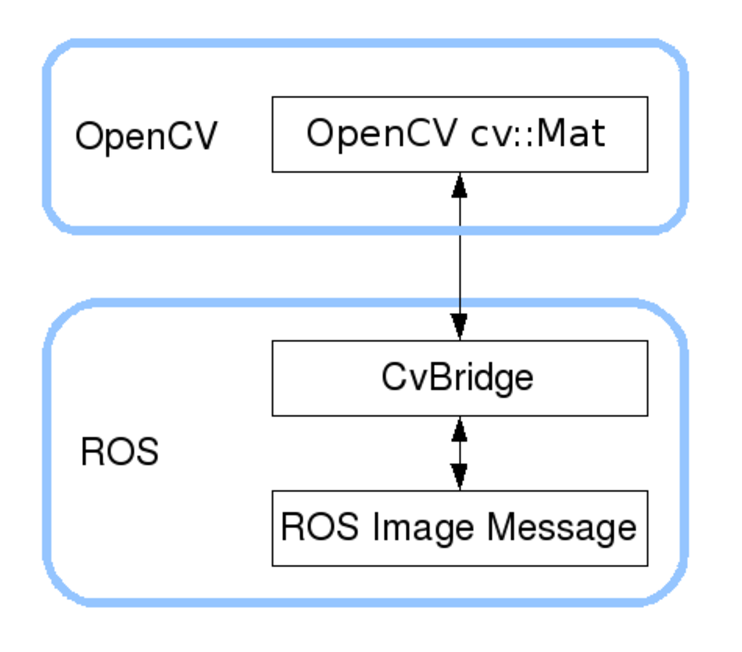
\includegraphics[width=0.6\textwidth]{Capitulo1/Fig1.eps}       
        \captionof{figure}{Uso de una gimbal para una IMU ~\cite{InertialNavigation} }\label{Fig1}
    \end{center}
    En esta aplicación, la Unidad de medición inercial (IMU) está equipada con tres 
    giroscopios montados ortogonalmente para detectar la rotación alrededor de todos 
    los ejes en el espacio tridimensional. Las salidas giroscópicas accionan motores 
    que controlan la orientación de los tres gimbal según sea necesario para mantener 
    la orientación de la IMU.

    \item \textbf{Motores de cohete}\\
    En la propulsión de naves espaciales, los motores de cohetes generalmente se 
    montan en un par de gimbals para permitir que un solo motor logre el empuje 
    sobre los ejes de inclinación y guiñada; o, a veces, solo se proporciona un eje 
    por motor. Para controlar el giro, se utilizan motores gemelos con señales de 
    control de inclinación diferencial o guiñada para proporcionar torque sobre el 
    eje de balanceo del vehículo.\\
    Uno de los motores más famosos es el J-2X.Es un motor de cohete avanzado altamente 
    eficiente y versátil con las características ideales de empuje y rendimiento para 
    impulsar la etapa superior del espacio de la NASA.~\cite{NASA}
    \begin{center}
        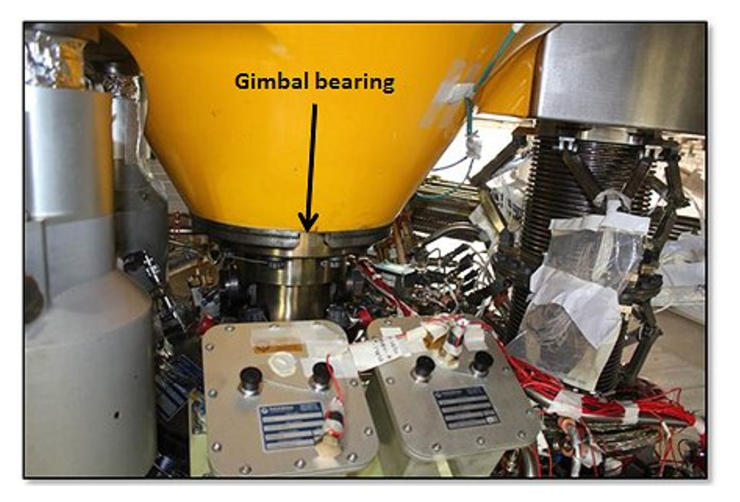
\includegraphics[width=0.6\textwidth]{Capitulo1/Fig2.eps}       
        \captionof{figure}{Uso de una gimbal en un motor de propulsión ~\cite{NASA2JX} }\label{Fig2}
    \end{center}

    \item \textbf{Entrenamiento para astronautas}\\
    Sistema de simulación de maniobras de tipo caída que se pueden encontrar en el vuelo espacial
    fue creado por la NASA y era conocido como "the gimbal rig,".
    Tres jaulas tubulares de aluminio podrían girar por separado o en combinación para 
    dar movimientos de balanceo, cabeceo y guiñada a velocidades de hasta 30 
    revoluciones por minuto, mayores que las esperadas en vuelos espaciales reales. 
    Los chorros de gas nitrógeno, unidos a las tres jaulas, controlaron el movimiento.
    Desde el 15 de febrero hasta el 4 de marzo de 1960, la plataforma de cardán 
    proporcionó una capacitación valiosa para los siete astronautas del Proyecto 
    Mercurio. Cada uno experimentó unas cinco horas de tiempo de vuelo simulado.
    ~\cite{MERCURY}
    \begin{center}
        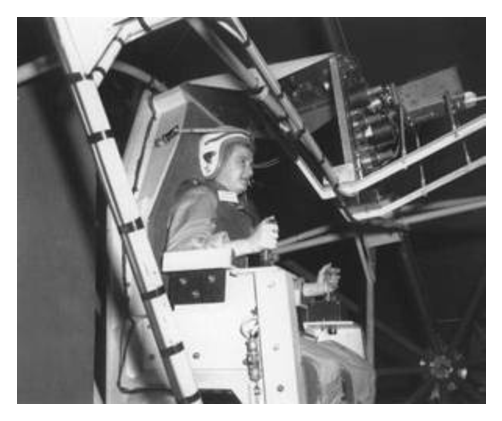
\includegraphics[width=0.6\textwidth]{Capitulo1/Fig3.eps}       
        \captionof{figure}{Jerrie Cobb, uno de los Mercury 13, da un giro en la plataforma gimbal.
        Créditos: NASA }\label{Fig3}
    \end{center}

    \item \textbf{Estabilizador de Camaras}\\
    Los gimbals también se utilizan para montar todo, desde lentes de cámara pequeñas 
    hasta telescopios fotográficos grandes.\\
    En los equipos de fotografía portátiles, se utilizan gimbals de un 
    solo eje para permitir un movimiento equilibrado de la cámara y las lentes. 
    Esto resulta útil en la fotografía semi-profesional, así como en cualquier otro 
    caso en el que se adopten teleobjetivos muy largos y pesados: un eje de la gimbal 
    gira un lente alrededor de su centro de gravedad, lo que permite una manipulación 
    fácil y suave mientras se rastrea a los sujetos en movimiento.\\
    Los montajes de gimbal muy grandes en forma de montajes de altitud-altitud de 2 o 3 ejes 
    se utilizan en la fotografía satelital con fines de seguimiento.\\
    En la década de 1970, el director de fotografía estadounidense Garrett Brown tuvo 
    una idea simple pero revolucionaria: hacer un dispositivo que pudiera suavizar las 
    tomas de acción manuales. 
    \begin{center}
        \includegraphics[width=0.5\textwidth]{Capitulo1/Fig4.eps}       
        \captionof{figure}{Primer uso de la steadicam}\label{Fig4}
    \end{center}

    El resultado es el Steadicam (Que cumple con los principios físicos de la gimbal) \\
    Ganador de un Premio de la Academia, que hizo su debut cinematográfico en la 
    película "Bound for Glory", y se destacó en las películas "Rocky" y "The Shining"


\end{itemize}

\section{Contribuciones}
%%%%%%%%%%%%%%%%%%%%%%%%%%%%%%%%%%%%%%%%%%%%%%%%%%%%%%%%%%%%%%%%%%%%%%%%%
%                         Contribuciones                                %
%%%%%%%%%%%%%%%%%%%%%%%%%%%%%%%%%%%%%%%%%%%%%%%%%%%%%%%%%%%%%%%%%%%%%%%%%

\section{Alcances}
%%%%%%%%%%%%%%%%%%%%%%%%%%%%%%%%%%%%%%%%%%%%%%%%%%%%%%%%%%%%%%%%%%%%%%%%%
%¿Porque es relevante la solucion o mejora o implementacion.? ¿por que es novedosa? %
%%%%%%%%%%%%%%%%%%%%%%%%%%%%%%%%%%%%%%%%%%%%%%%%%%%%%%%%%%%%%%%%%%%%%%%%%


\section{Estructura de la tesis}
\chapter{Marco Téorico}
\cleanchapterquote{Never memorize something that you can look up.}{Albert Einstein}{(Theoretical physicist)}


En este capitulo desarrolla la teoría que fundamenta el proyecto de investigación con base
en el problema previamente descrito.\\
Antes de entrar a la teoría es necesario entender cuales son las fases del proyecto y
el porque de ellas.
La siguiente imagen muestra la similitud entre el sistema de adquisición de datos
de un humano y la de un sistema digital.
\begin{center}
	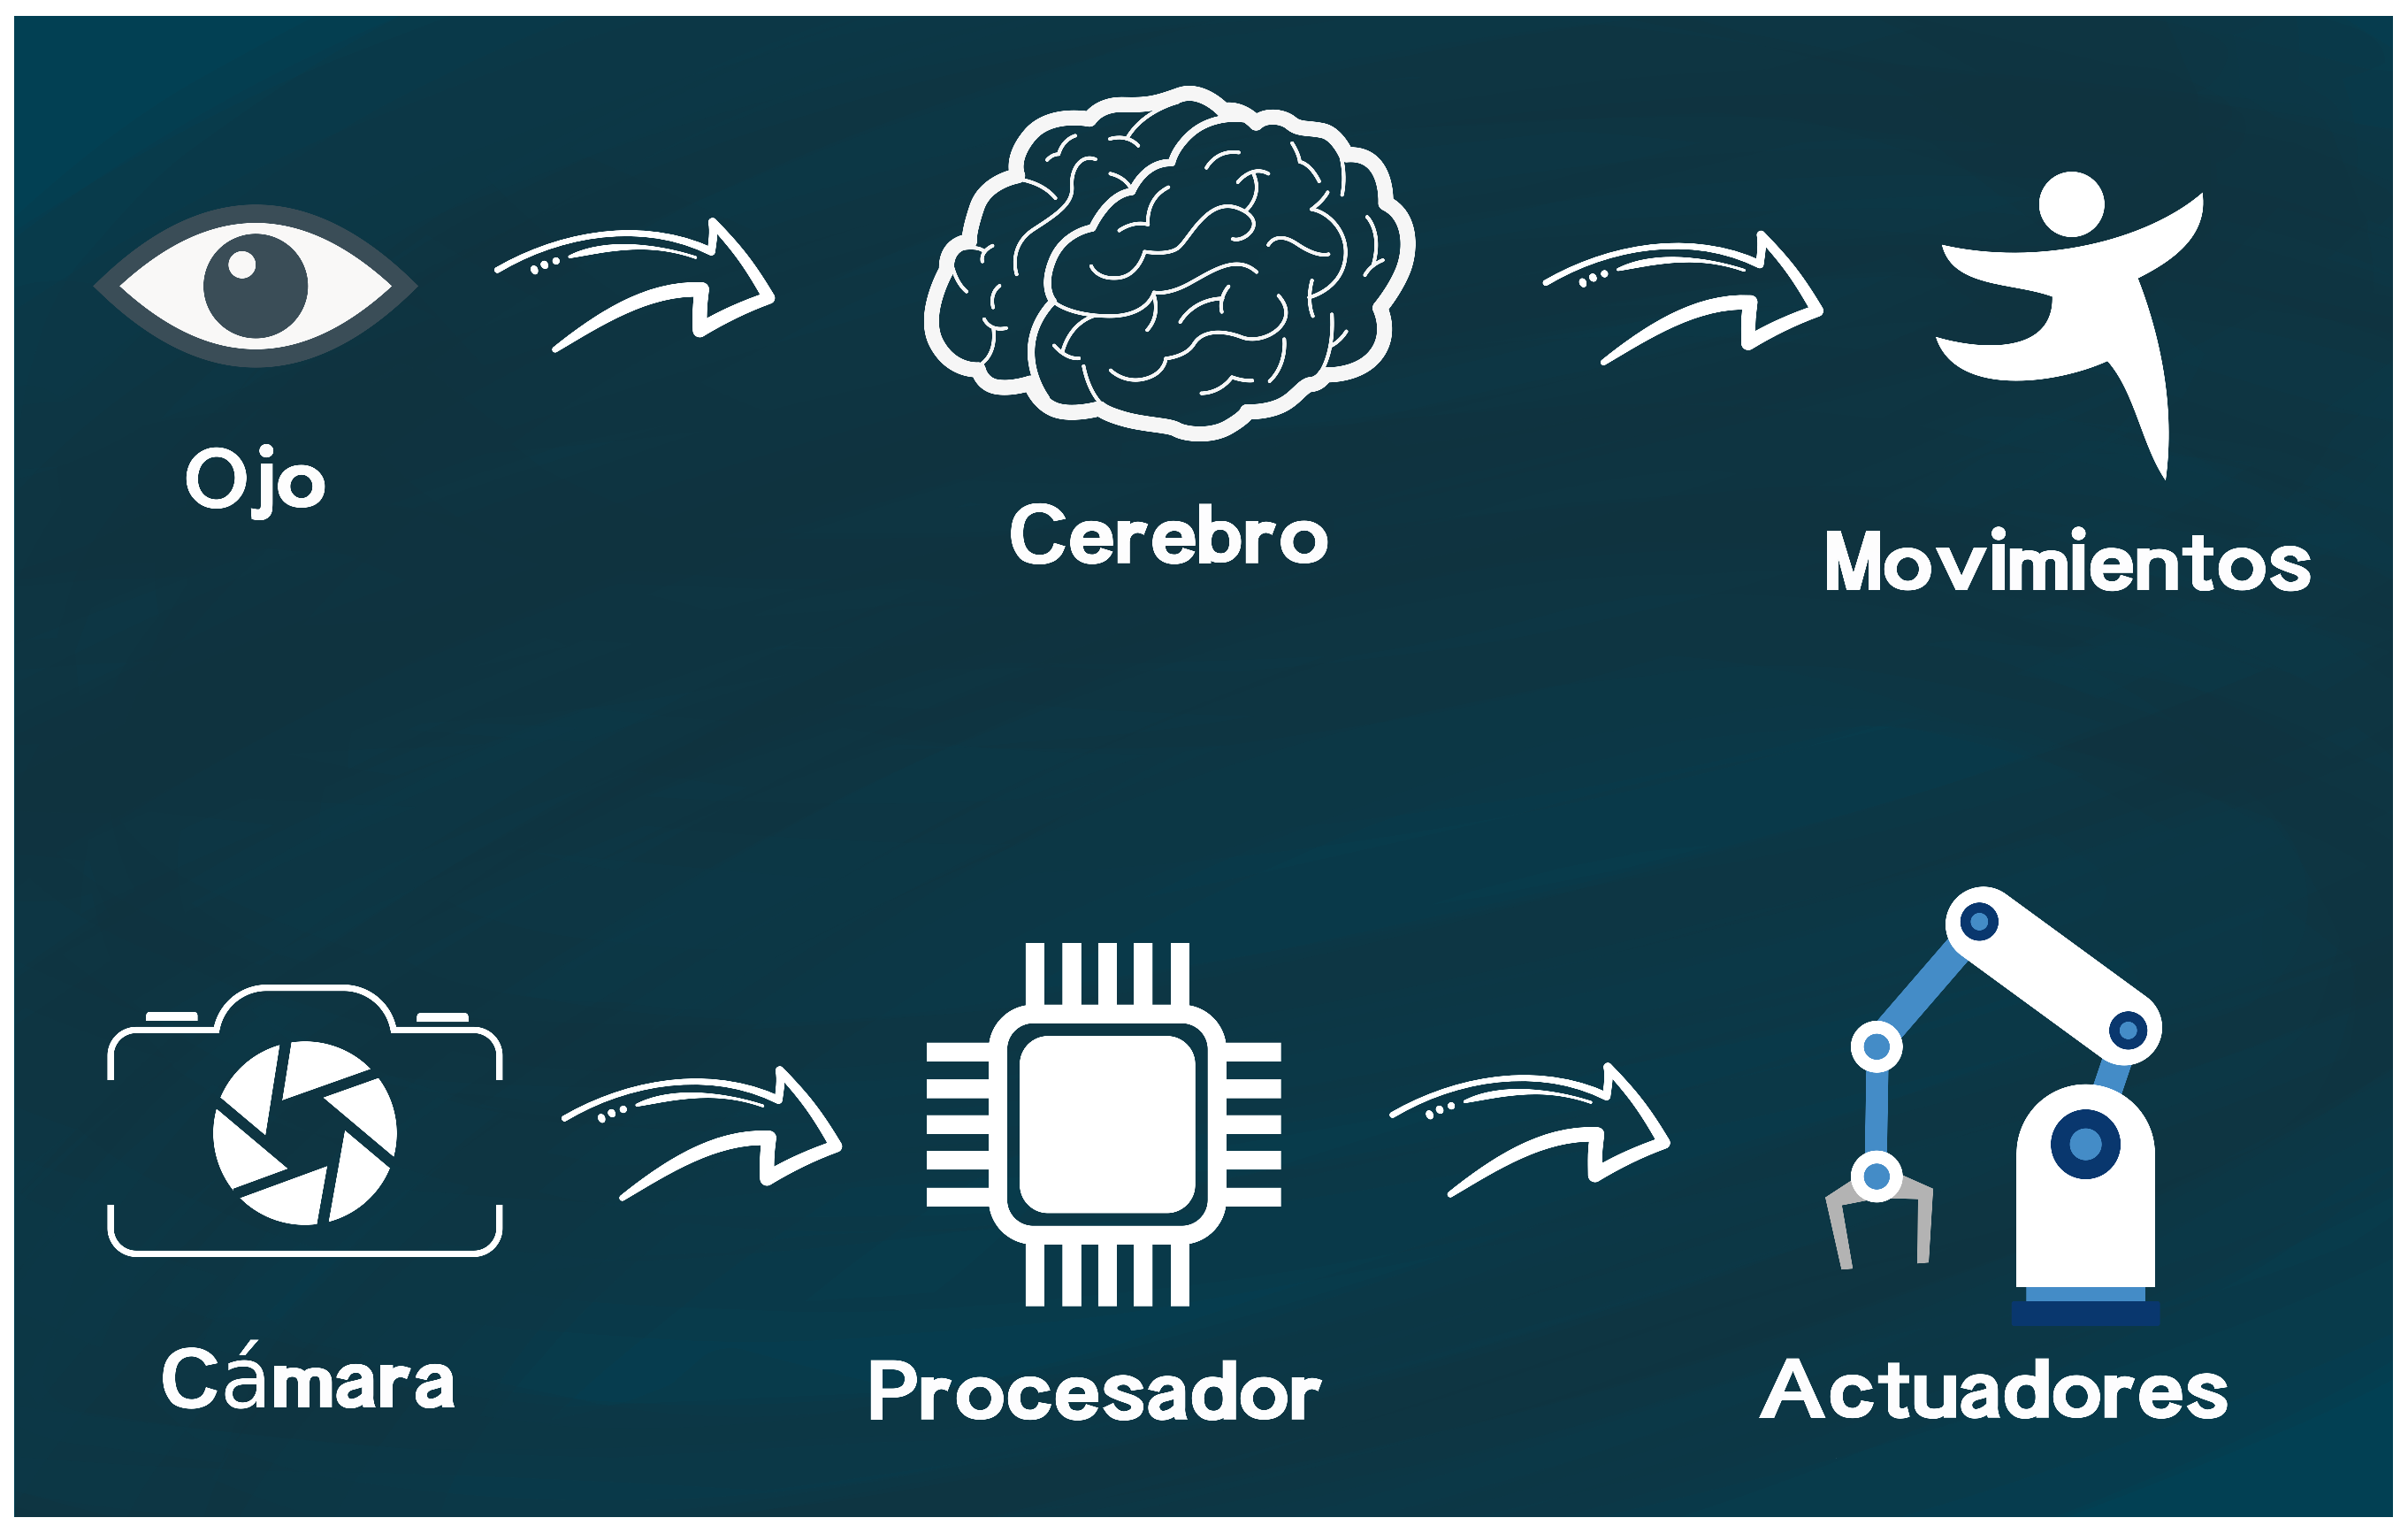
\includegraphics[width=0.65\textwidth]{Contenido/Cuerpo/Capitulo2/Fig1.eps}
	\captionof{figure}{Similitudes entre humano y computadora}
	\label{fig:MarcoTeorico:Fig1}
\end{center}
Donde se observa un diagrama de flujo que empieza con la adquisición de datos, en este
caso la captura de una imagen, posterior se hace un procesamiento, es decir, se le da
sentido a los datos, y finalmente se hace una acción con base en la tarea que el procesador
ha generado.


% **************************************************************************************************************************
% **************************************************************************************************************************
% NUEVA SECCION 
% OPTICA
% **************************************************************************************************************************
% **************************************************************************************************************************
\section{Óptica}

La visión artificial surge de un amplio estudio probabilístico y matemático del
procesamiento de imágenes digitales, pero sobre todo de análisis humanos y de la
intuición ya que de estas últimas el ingeniero hace selección de entre una u otra
técnica. Esta elección se basa usualmente en juicios visuales subjetivos.\\
Entender los conceptos básicos de la percepción humana es entonces pertinente, donde
la Óptica nos ayudará a entender mejor como es que el ojo humano percibe y como lo
hace una cámara. \\
La función de la óptica de una cámara es captar los rayos luminosos y concentrarlos
sobre el sensor sensible de la cámara de vídeo. Después de determinar el tipo de
iluminación que mejor se adecua al problema, la elección de una óptica u otra influirá
en la calidad de la imagen y el tamaño de los objetos.

% ----------------------------------------------------------------------------------------------------------------------------
% NUEVA SUBSECCION
% ----------------------------------------------------------------------------------------------------------------------------
\subsection{Descripción general del sistema visual humano}
La luz entra al ojo y estimula los sensores en la parte posterior.
La señal que se crea luego viaja a través del nervio óptico, cruzando el
nervio que proviene del otro ojo y llega a un órgano, en el interior del
cerebro en el área del tálamo, llamado núcleo geniculado lateral (LGN).
Las salidas de la LGN se envían a la corteza visual en la parte posterior del cerebro.
La corteza visual es quizás la parte más compleja del cuerpo humano. Es el lugar en el
cerebro donde tiene lugar la mayor parte del procesamiento visual.\cite{Book:Anil2008}
\begin{center}
	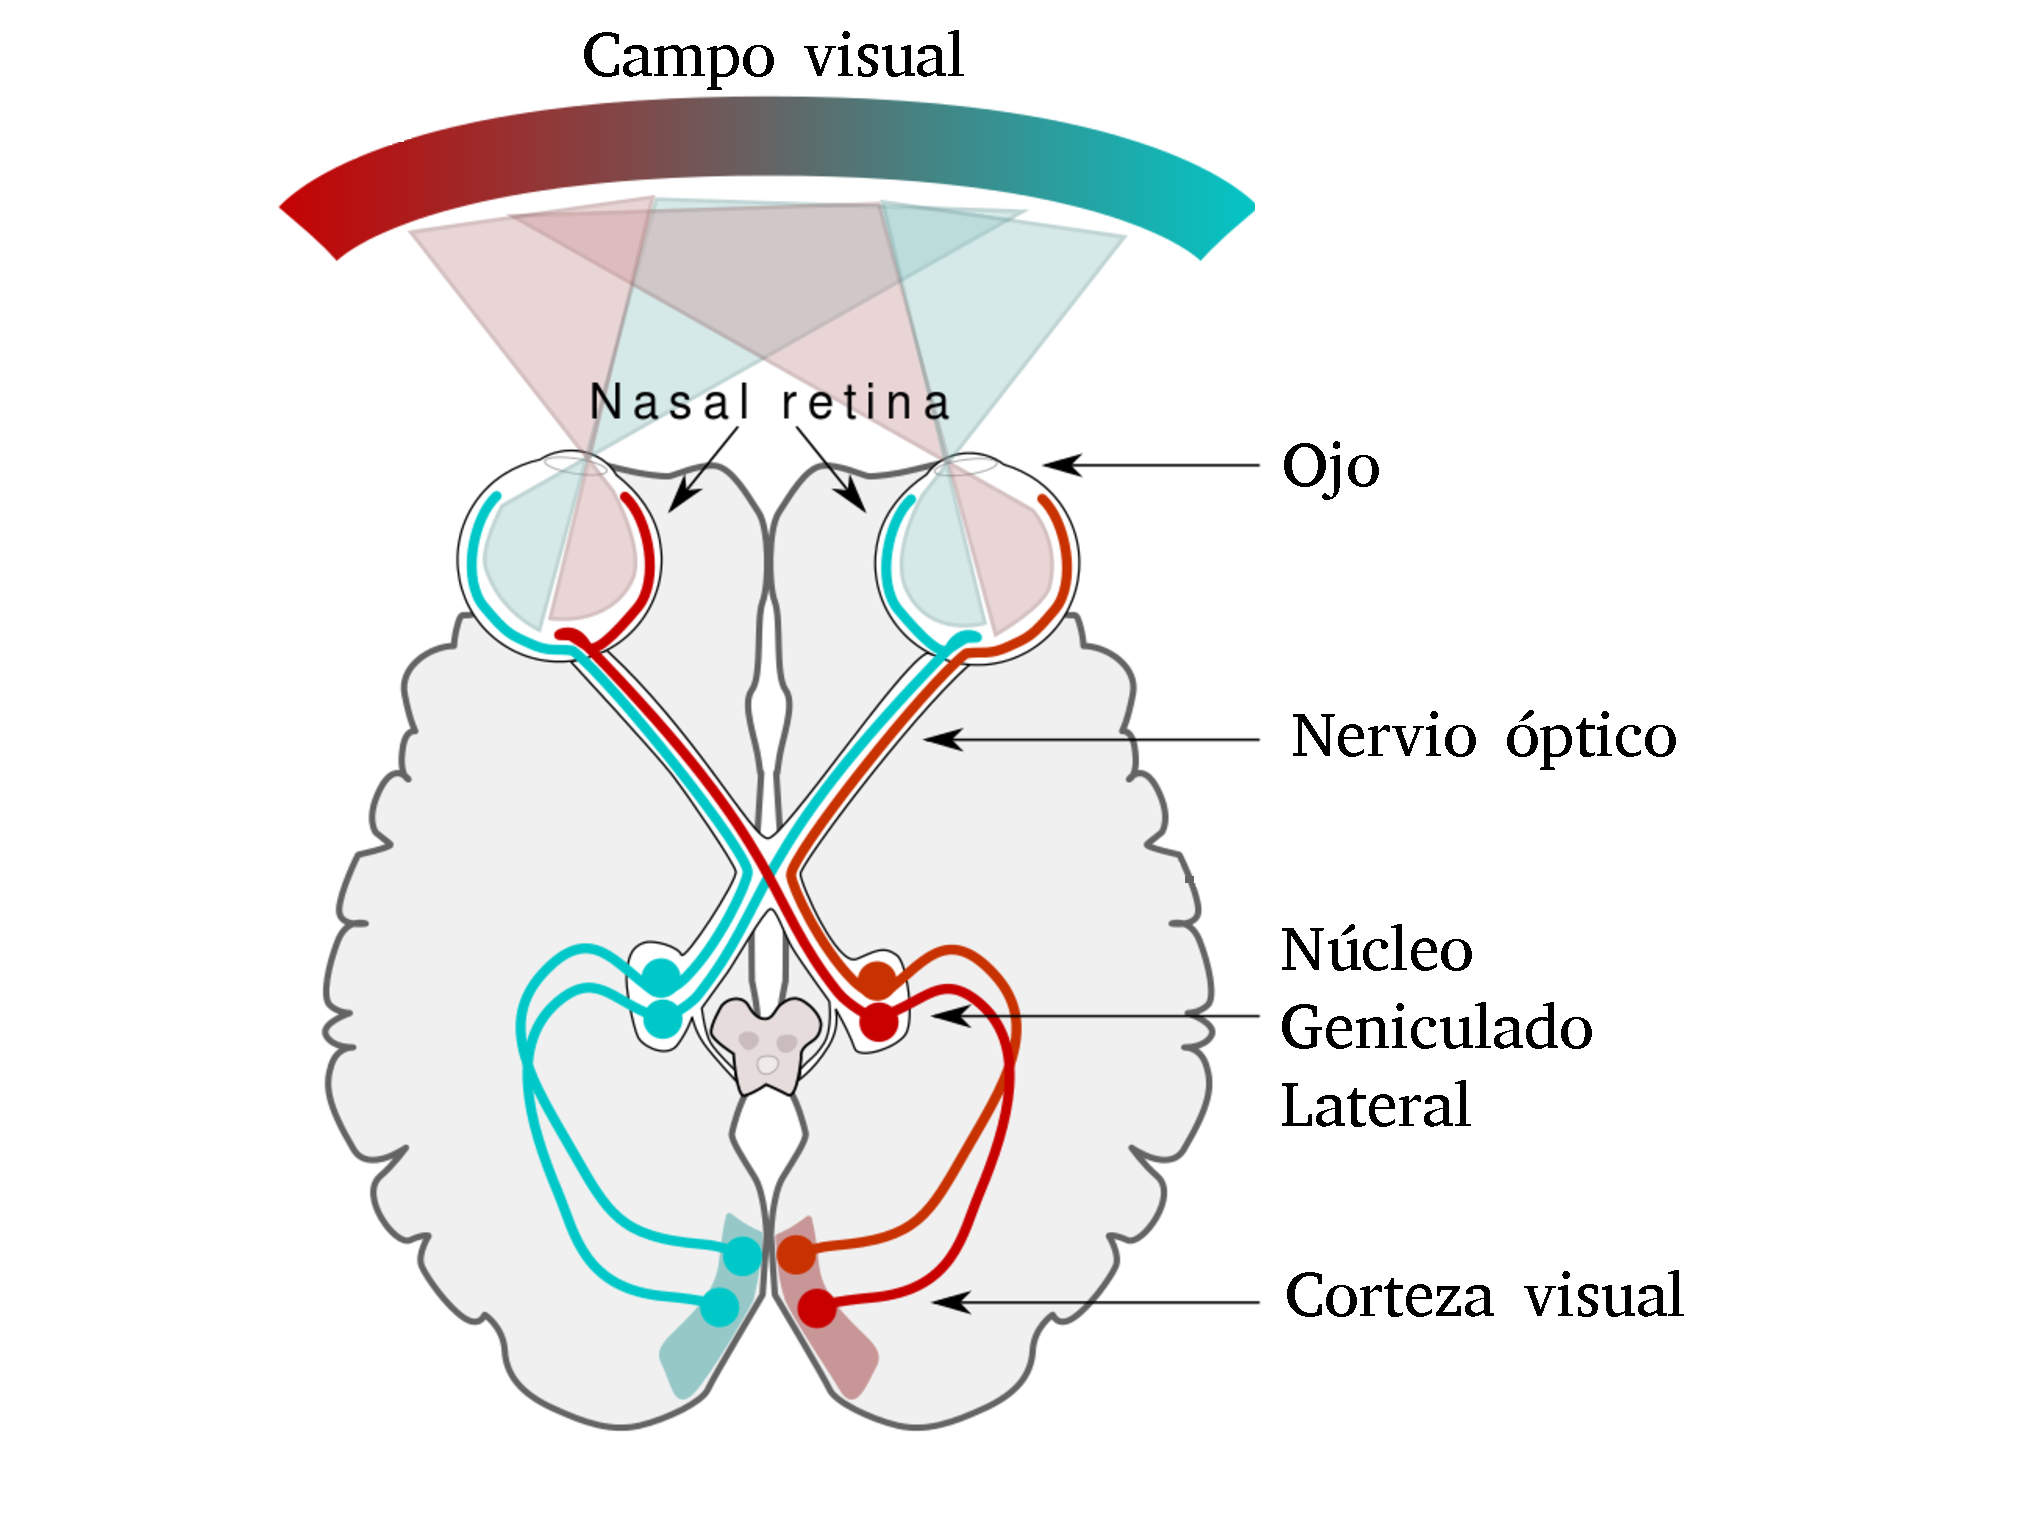
\includegraphics[width=0.55\textwidth]{Contenido/Cuerpo/Capitulo2/Fig1_1.eps}
	\captionof{figure}{El camino que sigue la señal óptica dentro de la cabeza humana.}
	\label{fig:MarcoTeorico:Fig2}
\end{center}
En términos generales, cuanto más nos alejamos del camino visual del ojo, menos
entendemos lo que está sucediendo.

% ----------------------------------------------------------------------------------------------------------------------------
% NUEVA SUBSECCION
% ----------------------------------------------------------------------------------------------------------------------------
\subsection{Estructura del ojo humano}
Es necesario abordar algunos conceptos basicos para entendernos en un
futuro, pero sobre todo comprender las similitudes del ojo humano y
la cámara, además de analizar limitaciones físicas de la vista humana
en los mismos términos que usaremos para nuestras imágenes digitales.\\
El ojo esta formado de dos componentes principales:
\begin{itemize}
	\item \textbf{Componentes ópticos:} \\Permiten la formación de la imagen en la retina y son los
	      siguientes: la córnea, el cristalino, la pupila, el humor acuoso y el humor vítreo que
	      permiten la formación de una imagen en la retina.
	\item \textbf{Componentes neurológicos:}\\ son los que transforman la información óptica en
	      eléctrica y transmiten la información al cuerpo geniculado lateral. Estos componentes
	      son la retina y el nervio óptico.
\end{itemize}
\begin{itemize}
	\item Cornea: La córnea es una estructura del ojo que permite el paso de la luz
	      desde el exterior al interior del ojo y protege el iris y el cristalino. Posee
	      propiedades ópticas de refracción y para garantizar su función debe ser transparente
	      y es necesario que mantenga una curvatura adecuada.
	\item Esclerótica: Es el recubrimiento exterior blanco del ojo. La esclerótica le da
	      su color blanco al globo ocular.
	\item Coroides: Es la capa de vasos sanguíneos y tejido conectivo entre la parte blanca del ojo y la retina (en la parte posterior del ojo). Es parte de la úvea y suministra los nutrientes a las partes internas del ojo.
	\item Cuerpo ciliar: Es una estructura circular que es una prolongación del iris, la
	      parte de color del ojo. También contiene el músculo ciliar, el cual cambia la forma
	      del cristalino cuando los ojos se enfocan en un objeto cercano. Este proceso se
	      denomina acomodación.
	\item Diafragma Iris: que se expande o contrae para controlar la cantidad de luz que
	      entra en el ojo. La apertura central del iris, llamada pupila, varía su diámetro de 2
	      a 8mm. El frente del iris contiene el pigmento visible del ojo, y la parte trasera
	      contiene un pigmento negro.
	\item Cristalino: El cristalino es “la lente” del ojo y sirve para enfocar, ayudado
	      por los músculos ciliares. El cristalino es una lente que actúa como una lente
	      biconvexa, lenticular, flexible y avascular, cuya principal función es la de enfocar
	      los objetos en las distintas distancias correctamente.
	\item Retina: Es la capa de tejido sensible a la luz que se encuentra en la parte
	      posterior globo ocular. Las imágenes que pasan a través del cristalino del ojo se
	      enfocan en la retina. La retina convierte entonces estas imágenes en señales eléctricas
	      y las envía por el nervio óptico al cerebro.
\end{itemize}
\cite{Book:Jose2005}

% ----------------------------------------------------------------------------------------------------------------------------
% NUEVA SUBSECCION
% ----------------------------------------------------------------------------------------------------------------------------
\subsection{Formación de imágenes en el ojo}
El sentido de la vista en las personas tiene un funcionamiento complejo y
necesita de dos elementos básicos: El ojo y el cerebro.\\
La luz es el tercer elemento más destacado en la visión. Sin ella somos
incapaces de ver. Dentro del ojo se sigue una seria de pasos para poder capturar
una imagen con base en la luz disponible.
\begin{itemize}
	\item La luz pasa a través de la córnea y llega a la pupila que se contrae o
	      expande según su intensidad. La pupila será más pequeña cuanta más luz haya para
	      evitar deslumbramientos.
	\item El cristalino del ojo será quien proyecte las imágenes enfocadas en la retina.
	      Puede aplanarse o abombarse según lo cerca o lejos que esté el objeto que veamos.
	\item La retina recibe la imagen invertida en sus paredes. La luz estimula los
	      conos y los bastones quienes transforman esa información en impulsos nerviosos.
	      Esta electricidad se trasladará al cerebro a través del nervio óptico.
\end{itemize}
\begin{center}
	\includegraphics[width=0.65\textwidth]{Contenido/Cuerpo/Capitulo2/Fig1_3.eps}
	\captionof{figure}{Formación de una imagen en el ojo}
	\label{fig:MarcoTeorico:Fig3}
\end{center}
El cerebro es quien realmente ve las imágenes. Endereza la imagen invertida de la
retina e interpreta la información de color, tamaño, posición, etc.
La distancia entre el centro del
cristalino y la retina (que llamaremos distancia focal), varía de
aproximadamente 17mm a 14mm.\cite{Book:Jose2005}

\subsubsection{Fotorreceptores}
Los fotorreceptores son células especializadas de la retina del ojo responsables de
convertir la luz en señales que son enviadas al cerebro. Los fotorreceptores nos dan
la visión de color y la visión nocturna.\cite{WEB:American}

% ----------------------------------------------------------------------------------------------------------------------------
% NUEVA SUBSECCION
% ----------------------------------------------------------------------------------------------------------------------------
\subsection{Camara digital}
La cámara digital es uno de los cambios más importantes en esta era de la digitalización
de la información. Es un invento tan revolucionario y que dista tanto de su predecesor
análogo.\\
Las cámaras digitales producen imágenes capturando o grabando las características de
la luz de una escena o sujeto. Las partes principales de la cámara que participan en
el proceso son el cuerpo de la cámara, el obturador de la cámara, la lente de la cámara,
la apertura de la lente y el sensor de imagen de la cámara. \cite{WEB:CameraWorks}

% ----------------------------------------------------------------------------------------------------------------------------
% NUEVA SUBSECCION
% ----------------------------------------------------------------------------------------------------------------------------
\subsection{Componetes de la camara}
\begin{itemize}
	\item \textbf{Lente: }El objetivo de la lente de la cámara es enfocar y dirigir
	      la luz entrante. La lente de la cámara consta de una o más piezas de vidrio o
	      plástico de forma precisa llamadas elementos. La luz que entra por los elementos
	      se "dobla" o se dirige al sensor de imagen donde se captura la información sobre
	      la luz.
	\item \textbf{Obturador:} Sistema mecánico o electrónico que permite el paso de la
	      luz a través del sistema óptico  durante un tiempo determinado.
	\item \textbf{Diafragma: }Sistema mecánico o electrónico que gradúa la mayor o
	      menor intensidad de luz que debe   pasar durante el tiempo que está abierto el
	      obturador. En nuestro ojo la pupila se encarga de hacer esa función.
	\item \textbf{Sistema de enfoque: }Gradúa la posición del  objetivo, para que la
	      imagen se forme totalmente donde  está la placa sensible. Su función es similar a
	      la que realiza el cristalino en el ojo.
	\item \textbf{Sensor: }En el ojo, la retina es la parte a la que llega la luz
	      antes de transformarse en señales eléctricas. Si buscamos en la cámara fotográfica
	      un elemento que se asemeje nos encontramos con los sensores CCD o CMOS. Se
	      puede decir que estos dispositivos son los encargados de transformar la luz en
	      carga eléctrica para crear cada pixel de la imagen.\\
	      El sensor de imagen tiene una cuadrícula con millones de elementos microscópicos
	      de información de luz llamados "fotosites".
	      Cada una de estas fotositas se conoce mejor como píxeles.
\end{itemize}
\begin{center}
	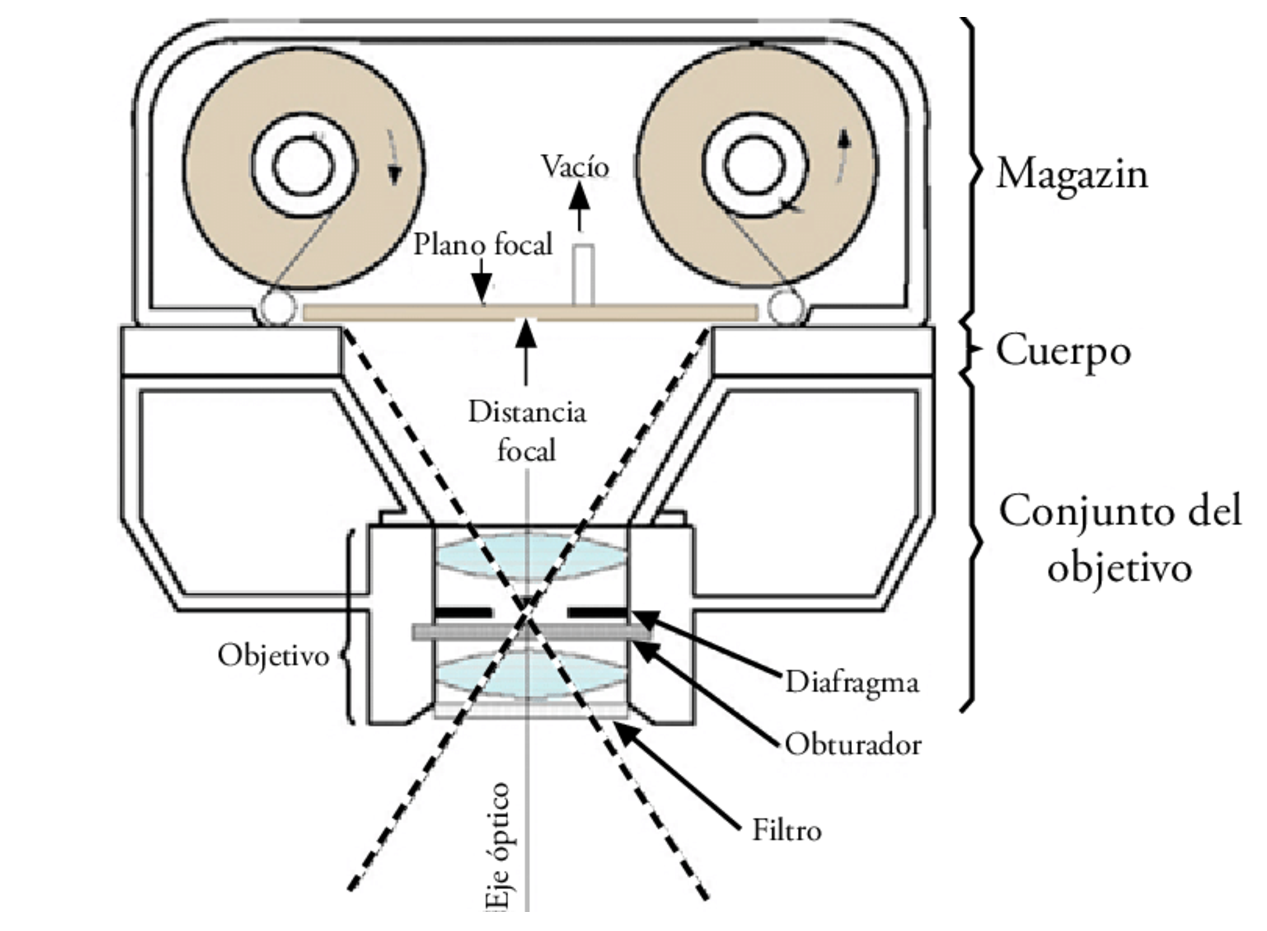
\includegraphics[width=0.45\textwidth]{Contenido/Cuerpo/Capitulo2/Fig1_5.eps}
	\captionof{figure}{Componentes de la camara}
	\label{fig:MarcoTeorico:Fig4}
\end{center}

% ----------------------------------------------------------------------------------------------------------------------------
% NUEVA SUBSECCION
% ----------------------------------------------------------------------------------------------------------------------------
\subsection{Formación de la imagen en la camara}
En una cámara fotográfica se recibe la luz que traspasa el diafragma, pasa por los
cristales de la cámara hasta llegar al CCD(Charge Coupled Device o, en español,
Dispositivo de Carga Acoplada) o sensor, que es donde se forma la imagen correcta y se
envía al procesador.\\
Algo similar pasa en el ojo, la pupila es el diagrama natural que filtra la luz que
entra en el ojo, pasa por la lente (el cristalino)  que converge los rayos hasta
llegar a la retina, que es la estructura que tiene las células fotosensibles y dónde
se produce la imagen, y a través del nervio óptico se transporta la información al
cuerpo geniculado, que es la parte del cerebro donde se produce la visión.
\begin{center}
	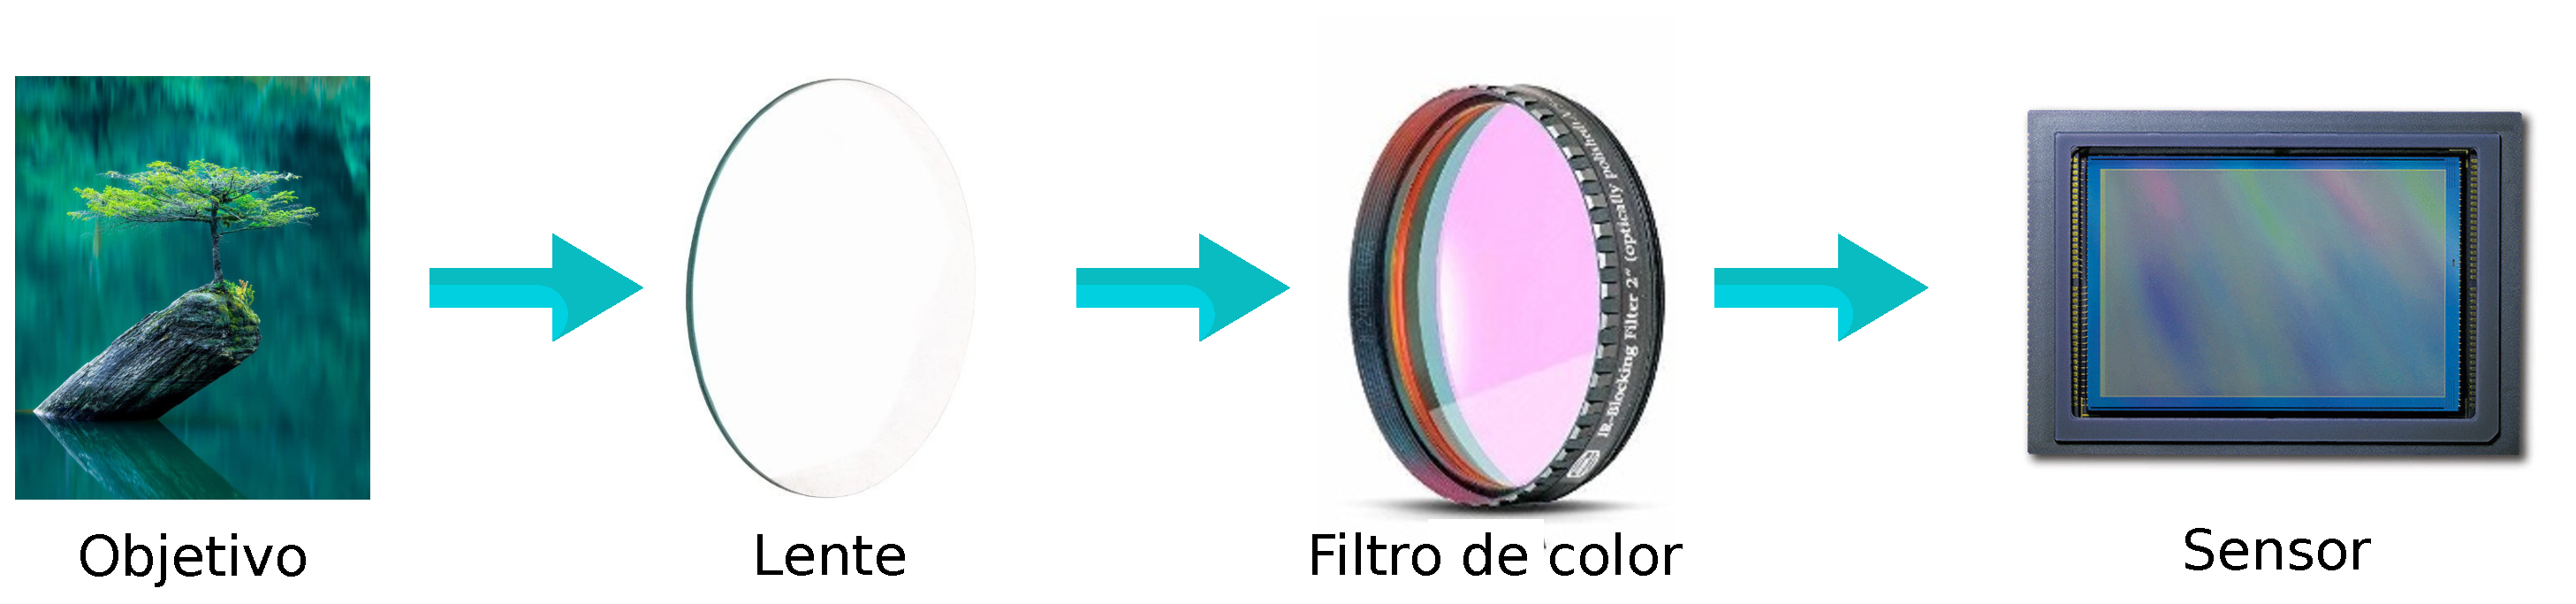
\includegraphics[width=0.7\textwidth]{Contenido/Cuerpo/Capitulo2/Fig1_6.eps}
	\captionof{figure}{Proceso general de captura de imagen por la cámara}
	\label{fig:MarcoTeorico:Fig5}
\end{center}

Cuando los rayos paralelos pasan a través de una lente convexa, convergen
hacia un punto que se denomina punto focal.\\
Realmente toda lente tiene dos puntos focales según la luz pase en un sentido o
en el opuesto. La distancia focal (mm, milímetros) es uno de los parámetros de los
objetivos de las cámaras. Llamamos longitud  focal de un objetivo a la distancia que
existe entre el sensor (plano focal) y la lente.\\
La distancia focal está también relacionada con la cantidad de luz
refractada por la lente. Es el denominado factor de potencia D cuyo valor es la inversa
de la distancia focal y su unidad de medida la dioptría.\\
Otro valor que se encontrará en toda óptica es el número F. Este parámetro
indica la relación entre la distancia focal y el diámetro del diafragma:
\begin{equation}
	F = \frac{f}{D}
\end{equation}
\begin{center}
	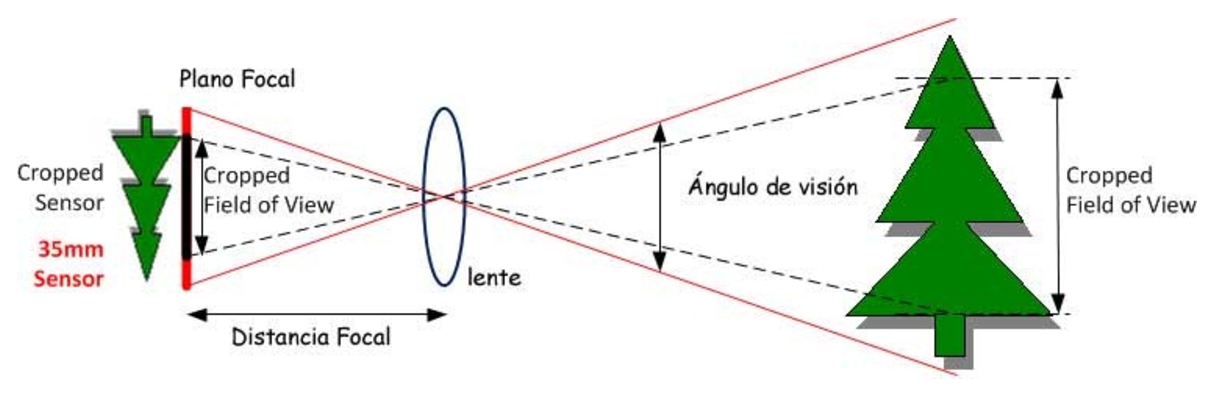
\includegraphics[width=0.75\textwidth]{Contenido/Cuerpo/Capitulo2/Fig1_4.eps}
	\captionof{figure}{Captura de imagen}
	\label{fig:MarcoTeorico:Fig6}
\end{center}
Indica la cantidad de luz (brillantez) que se deja pasar por el objetivo y se puede regular
mediante un anillo presente en la montura de la óptica.\\
En las ópticas habrá que tener por
tanto en cuenta su F mínimo, que indicará la máxima cantidad de luz que puede
atravesar la óptica y que tendrá que estar en concordancia con la sensibilidad de la
cámara.

% ----------------------------------------------------------------------------------------------------------------------------
% NUEVA SUBSECCION
% ----------------------------------------------------------------------------------------------------------------------------
\subsection{Cálculo de la imagen}
La imagen de un objeto en una lente convergente se obtiene geométricamente aplicando las siguientes reglas:
\begin{itemize}
	\item \textbf{Regla 1}\\
	      Cualquier rayo incidente paralelo al eje principal en la zona objeto sale pasando por el foco principal en la zona imagen
	      \begin{center}
		      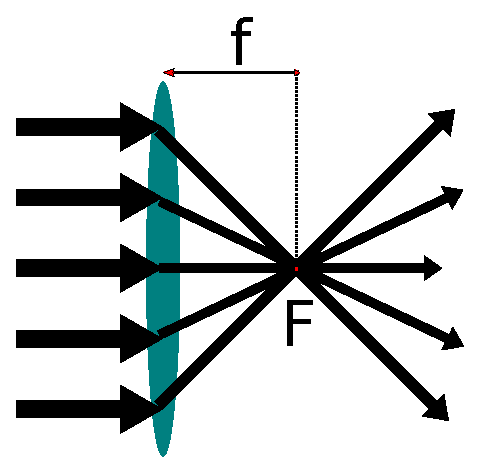
\includegraphics[width=0.25\textwidth]{Contenido/Cuerpo/Capitulo2/Fig1_7.eps}
		      \captionof{figure}{Regla 1}
		      \label{fig:MarcoTeorico:Fig7}

	      \end{center}
	\item \textbf{Regla 2}\\
	      Cualquier rayo incidente que pasa por el centro de la lente sale con la misma dirección, es decir, no sufre desviación
	      \begin{center}
		      
\includegraphics[width=0.2\textwidth]{Contenido/Cuerpo/Capitulo2/Fig1_8.eps}
		      \captionof{figure}{Regla 2}
		      \label{fig:MarcoTeorico:Fig8}
	      \end{center}
	\item \textbf{Regla 3}\\
	      Cualquier rayo incidente que corta al eje principal en la zona objeto a la misma distancia que la distancia focal, sale
	      paralelo al eje principal en la zona imagen.
	      \begin{center}
		      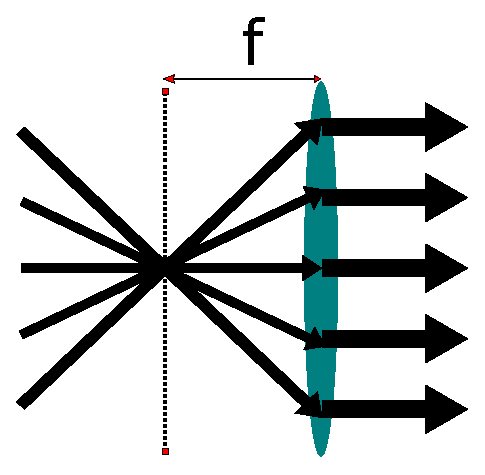
\includegraphics[width=0.25\textwidth]{Contenido/Cuerpo/Capitulo2/Fig1_9.eps}
		      \captionof{figure}{Regla 3}
		      \label{fig:MarcoTeorico:Fig9}
	      \end{center}

\end{itemize}
En la figura siguiente obtenemos la imagen P' del objeto P aplicando estas tres reglas. El rayo rojo es la primera regla;
el rayo verdaderamente es la segunda regla y el rayo azul la tercera. El punto P' donde se cortan los tres rayos es donde se forma la
imagen enfocada de P.
\begin{center}
	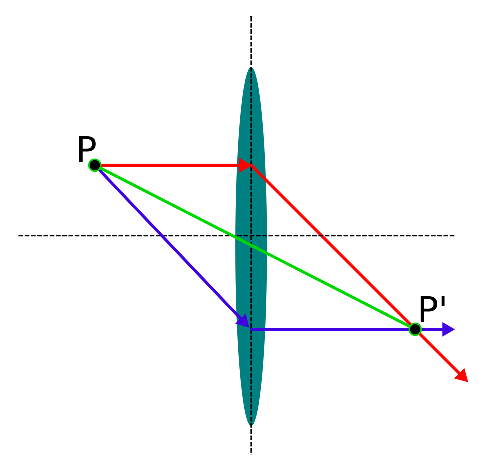
\includegraphics[width=0.35\textwidth]{Contenido/Cuerpo/Capitulo2/Fig1_10.eps}
	\captionof{figure}{Obtención geométrica de la imagen}
	\label{fig:MarcoTeorico:Fig10}
\end{center}
Estas tres reglas nos indican la trayectoria que seguirán tan sólo tres rayos de todos los que genera el objeto. La imagen vendrá
dada por el punto donde se intersecten esos rayos en la zona imagen.\\
En las ópticas habrá que tener por
tanto en cuenta su F mínimo, que indicará la máxima cantidad de luz que puede
atravesar la óptica y que tendrá que estar en concordancia con la sensibilidad de la
cámara. Por último sobre otro anillo similar se encuentra una escala graduada en metros,
que sirve para regular el enfoque según la distancia del objeto encuadrado. Al moverlo
el plano de elementos sensibles se aproxima a la lente para hacerlo coincidir con el de
formación de la imagen.\\
Este es el modelo denominado de la \textbf{lente fina}. La
lente fina es aquella en la que todo rayo que entra paralelo al eje óptico pasa por el foco
posterior de la lente y todo rayo que pasa por el foco anterior sale de la lente paralelo al
eje óptico.
\begin{center}
	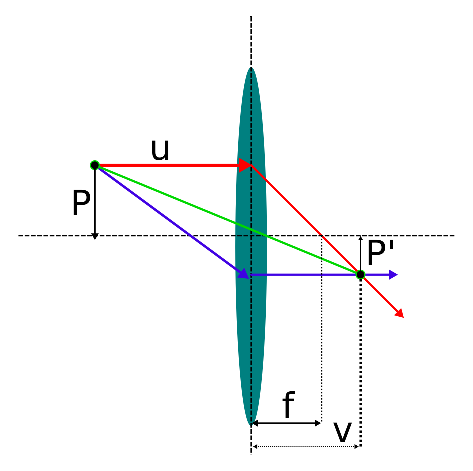
\includegraphics[width=0.35\textwidth]{Contenido/Cuerpo/Capitulo2/Fig1_11.eps}
	\captionof{figure}{Modelo de lente fina}
	\label{fig:MarcoTeorico:Fig11}
\end{center}

\subsection{Modelo de la cámara}
El modelo básico de la cámara también llamado
‘pin-hole’ representa la transformación de las
coordenadas de los puntos de la escena en las
coordenadas de la imagen. \cite{Paper::Ricolfe2008}\\
La siguiente imagen ilustra la proyeccion del punto \textbf{X} de ${\textbf{I\!R}^3}$ al punto \text{x}
de ${\textbf{I\!R}^2}$ 
\begin{center}
	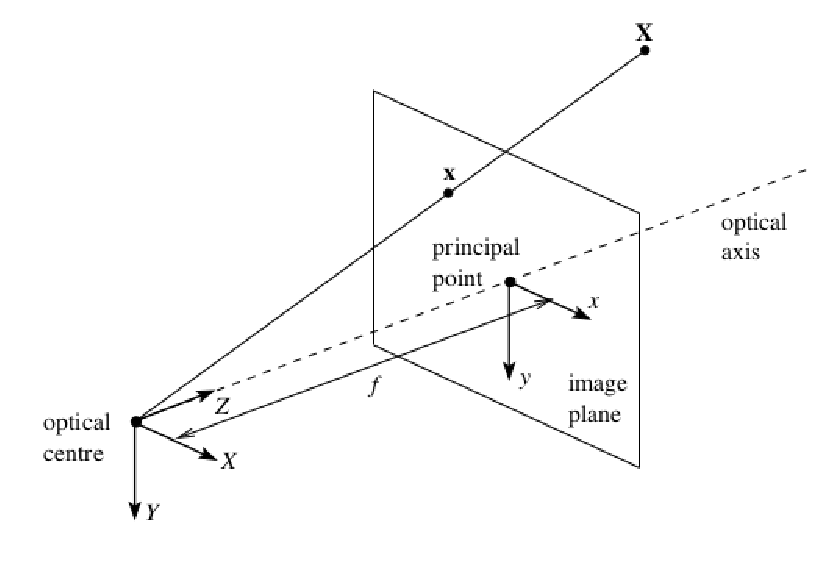
\includegraphics[width=0.35\textwidth]{Contenido/Cuerpo/Capitulo2/Fig19.eps}
	\captionof{figure}{Modelo pinhole tomado de \cite{Book:Geoffrey2006}}
	\label{fig:MarcoTeorico:Fig11}
\end{center}
Por triangulo semejantes podemos obtener las ecuaciones que relacionan un punto en el espacio con 
su proyección en la imagen.
\begin{equation}
	\textbf{x} = \frac{f}{Z}\textbf{X}
\end{equation}
\begin{equation}
	\textbf{y} = \frac{f}{Z}\textbf{Y}
\end{equation}
Queda aquí clara la perdida de una dimensión que se explicó en la introducción,
ya que todos los puntos cuya relación entre la coordenadas X y Z sea constante darán la
misma coordenada x en la imagen (igual con Y, Z e y).\cite{Book:Jose2005}\\
DEspejando de las ecuaciones anteriores obtenemos la distancia focal como
\begin{equation}
	f = Z \frac{\textbf{x}}{\textbf{X}}=ZM
\end{equation}
De donde M es el factor de magnificación.

% **************************************************************************************************************************
% **************************************************************************************************************************
% NUEVA SECCION 
% PROCESAMIENTO DE DATOS
% **************************************************************************************************************************
% **************************************************************************************************************************


\section{Procesamiento de datos}
En los seres humanos, el sistema visual recopila hasta el 80 por ciento de todos los datos sensoriales recibidos del entorno.
Para dar sentido a este diluvio de información óptica, las entradas visuales que son captadas y convertidas en señales
electroquímicas por los aproximadamente 130 millones de células sensibles a la luz en la retina se alimentan y procesan mediante
una compleja red de células nerviosas en el cerebro.\cite{WEB:Cerebro}
Es por lo anterior que la elección de un hardware que procese tanta información como lo hace el cerebro se vuele una tarea
prioritaria.

% ----------------------------------------------------------------------------------------------------------------------------
% NUEVA SUBSECCION
% ----------------------------------------------------------------------------------------------------------------------------
\subsection{Tarjeta procesadora}
La elección del hardware que será el cerebro de nuestro sistema es una tarea importante ya que de ello depende el éxito de
nuestro proyecto, y en estos tiempos el mercado ofrece una gran variedad de tarjetas procesadoras.
\begin{center}
	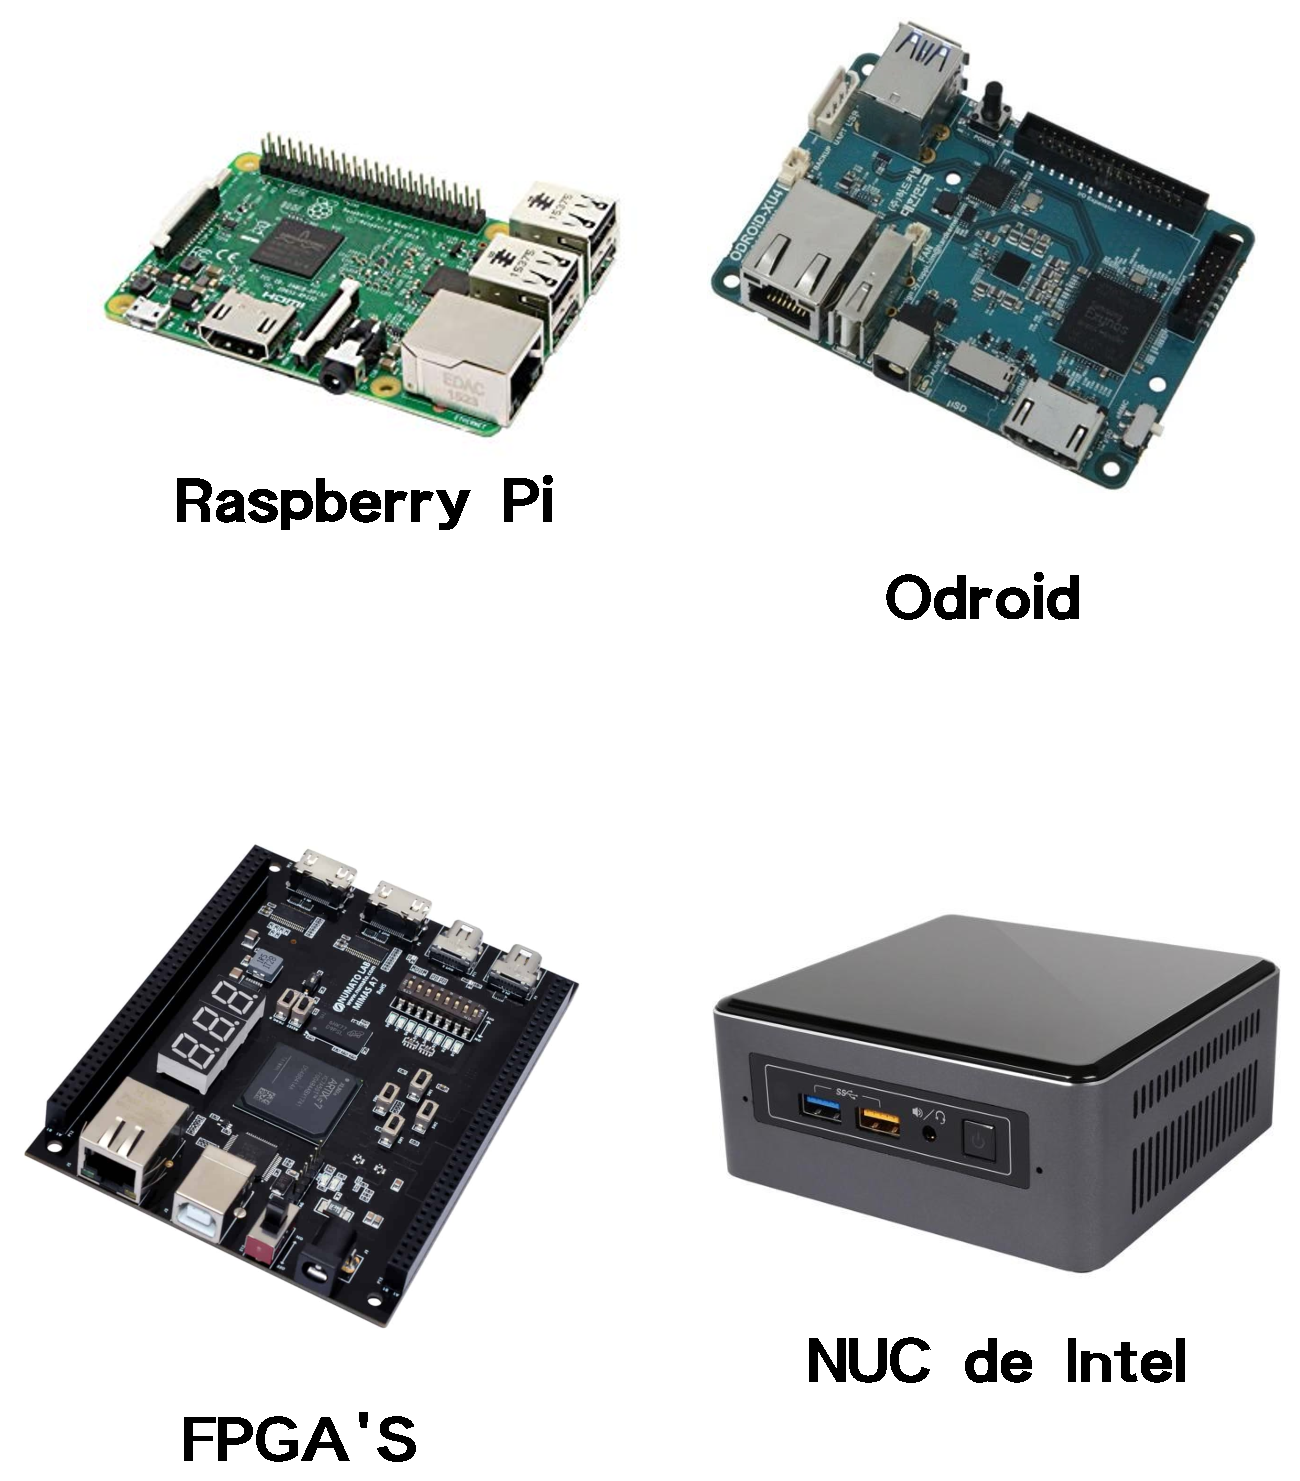
\includegraphics[width=0.35\textwidth]{Contenido/Cuerpo/Capitulo2/Fig7.eps}
	\captionof{figure}{Tarjetas procesadoras de datos}
	\label{fig:MarcoTeorico:Fig12}
\end{center}
Pasando desde un FPGA hasta un sistema totalmente completo como las NUC de Intel, pero para fines de este proyecto nos enfocaremos
solo en la hecha por HardKernel, la ODROID. Esto porque nos ofrece una capacidad de porcesamiento de datos apta para la visión
artificial y a un bajo costo.\\
Las placas de la serie Odroid son similares a Raspberry Pi, pero tiene una mejor
configuración y rendimiento. Se basa en la arquitectura ARM. \cite{Book:Lentin2018}
ODROID significa Open + Android. Es una plataforma de desarrollo tanto de
hardware como de software.\\
\textbf{Especificaciones técnicas en apéndice B.} \\
Con base en pruebas hechas por el proveedor, el modelo XU-4 resulta ser superior
a otras tarjetas de desarrollo del mercado.\\
Ejecutaron varios puntos de referencia para medir la potencia informática en el XU4.
Las mismas pruebas se realizaron en el Raspberry Pi 3 Modelo B, ODROID-C1 +, ODROID-C2
y ODROID-XU4.
Los valores de los resultados de la prueba se escalaron uniformemente para fines de
comparación. Se midió que la potencia informática del XU4 era ~ 7 veces más rápida que
la última Raspberry Pi 3 gracias a los núcleos 2Ghz Cortex-A15 y un ancho de banda de
memoria de 64 bits mucho mayor.\\
Compilar código en el XU4 es súper rápido. La memoria RAM DDR3 de 2 GB de
alto rendimiento es una ventaja adicional que permite compilar la mayoría de los
programas directamente en el XU4.\cite{WEB:HK2020}
\begin{center}
	
\includegraphics[width=0.65\textwidth]{Contenido/Cuerpo/Capitulo2/Fig6.eps}
	\captionof{figure}{Pruebas de performance}
	\label{fig:MarcoTeorico:Fig13}
\end{center}

% ----------------------------------------------------------------------------------------------------------------------------
% NUEVA SUBSECCION
% ----------------------------------------------------------------------------------------------------------------------------

\subsection{Sistema operativo}
Una vez elegida la tarjeta de desarrollo con la cual se estará trabajando para este
proyecto, el siguiente paso es escoger el sistema operativo que dará soporte a nuestro
sistema. Por defecto ODROID nos sugiere utilizar Ubuntu en su versión MATE.
\subsubsection{Ubuntu MATE}
Ubuntu MATE es una distribución de Linux gratuita y de código abierto y un derivado
oficial de Ubuntu.\\
Ubuntu es uno, si no es que el más grande, empleador de Linux en el mundo.Linux está en el
corazón de Ubuntu y hace posible crear sistemas operativos seguros, potentes y versátiles.\\
Ubuntu MATE toma el sistema operativo basado en Ubuntu y agrega el MATE Desktop.\\
Donde podemos definir MATE Desktop como una implementación de la metáfora del Desktop
hecha de un conjunto de programas que se ejecutan en la parte superior de un sistema
operativo de computadora, que comparten una interfaz gráfica de usuario (GUI) común.
Las GUI de escritorio ayudan al usuario a acceder y editar archivos fácilmente.\cite{WEB:Ubuntu}\\
Ubuntu soporta arquitecturas armhf, tipo de arquitectura de la odroid, además de optimizar
el sistema operativo sin sacrificar las ventajas que provee para una Computadora Portátil.

% ----------------------------------------------------------------------------------------------------------------------------
% NUEVA SUBSECCION
% ----------------------------------------------------------------------------------------------------------------------------

\subsection{ROS}
Un sistema de comunicación es a menudo una de las primeras necesidades que surgen al
implementar una nueva aplicación de robot. El sistema de mensajería integrado y
probado de ROS ahorra tiempo al administrar los detalles de la comunicación entre
los nodos distribuidos a través del mecanismo anónimo de publicación / suscripción.
Otro beneficio de usar un sistema de paso de mensajes es que te obliga a implementar
interfaces claras entre los nodos en tu sistema, mejorando así la encapsulación y
promoviendo la reutilización de código. La estructura de estas interfaces de mensajes
se define en el mensaje IDL (Lenguaje de descripción de interfaz).\\
Decidí usar ROS porque crear un software de robot verdaderamente robusto y de uso
general es difícil. Desde la perspectiva del robot, los problemas que parecen triviales
para los humanos a menudo varían enormemente entre instancias de tareas y entornos.
Hacer frente a estas variaciones es tan difícil que se necesita apoyo de un sistema
de comunicación.\\
ROS tiene tres niveles de conceptos: el nivel del sistema de archivos, el nivel del gráfico
de cómputo y el nivel de la comunidad. \cite{WEB:ROS}
\subsubsection{Nivel de sistemas de archivos de ROS}
Los conceptos de nivel de sistema de archivos cubren principalmente los recursos de ROS que
encuentra en el sistema, tales como:
\begin{itemize}
	\item \textbf{Paquetes}\\
	      Los paquetes son la unidad principal para organizar el software
	      en ROS. Un paquete puede contener procesos (nodos) de tiempo de ejecución de ROS,
	      una biblioteca dependiente de ROS, conjuntos de datos, archivos de configuración o
	      cualquier otra cosa que se organice conjuntamente de manera útil. Los paquetes son
	      el elemento de construcción más atómico y el elemento de lanzamiento en ROS. Lo
	      que significa que lo más granular que puede construir y lanzar es un paquete.
\end{itemize}
\subsubsection{Nivel de gráfico de cómputo ROS}
En términos generales, ROS sigue la filosofía de desarrollo de software de Unix
en varios aspectos clave. Esto tiende a hacer que ROS se sienta "natural" para los
desarrolladores que vienen de un entorno Unix, pero algo "críptico" al principio
para aquellos que han usado principalmente entornos de desarrollo gráfico en
Windows o Mac OS X.\cite{Book:Morgan2015}\\
Los sistemas ROS consisten en numerosos programas pequeños informáticos que se
conectan entre sí e intercambian mensajes continuamente. Estos mensajes viajan
directamente de un programa a otro.\\
Los conceptos básicos del gráfico de cómputo de ROS son nodos, mastaer,
servidor de parámetros, mensajes, servicios, topics y bags, los cuales
proporcionan datos al gráfico de diferentes maneras siguiendo la filosofia
antes descrita.
\begin{itemize}
	\item \textbf{Nodo}\\
	      los nodos son procesos que realizan cálculos. ROS está diseñado para ser modular
	      a nivel de nodo; un sistema de control de robot generalmente comprende muchos nodos.
	\item \textbf{Master}\\
	      Un programa intermedio que conecta nodos.
	      \begin{center}
		      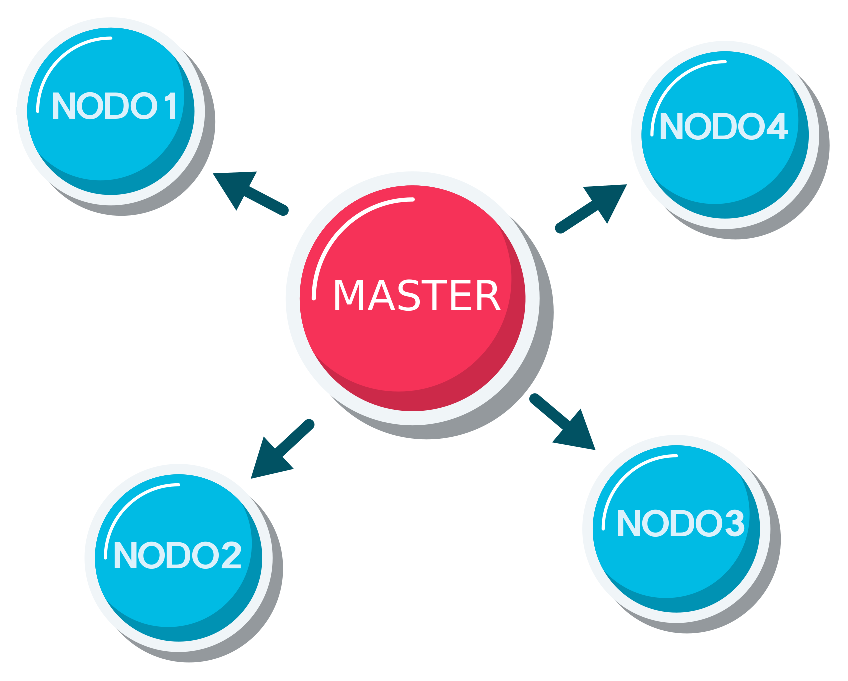
\includegraphics[width=0.5\textwidth]{Contenido/Cuerpo/Capitulo2/Fig2.eps}
		      \captionof{figure}{Nodos conectados al Master}
		      \label{fig:MarcoTeorico:Fig14}
	      \end{center}
	\item \textbf{Topics}\\
	      Los mensajes se enrutan a través de un sistema de transporte con semántica de
	      publicación / suscripción. Un nodo envía un mensaje al publicarlo en un topic
	      determinado. El topic es un nombre que se utiliza para identificar el contenido del
	      mensaje.
	      \begin{center}
		      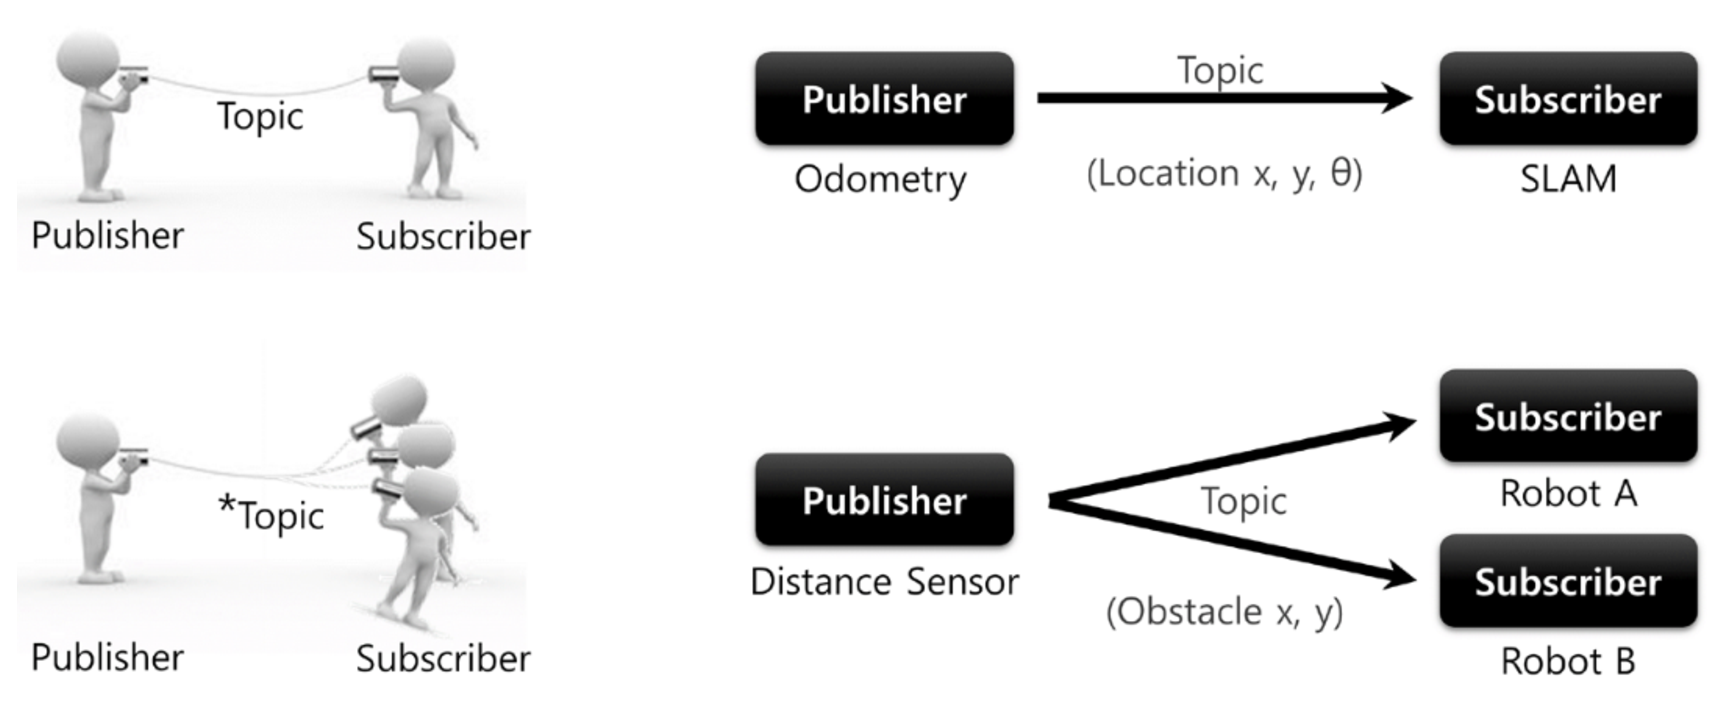
\includegraphics[width=0.75\textwidth]{Contenido/Cuerpo/Capitulo2/Fig3.eps}
		      \captionof{figure}{Representación grafica de Topics}
		      \label{fig:MarcoTeorico:Fig15}
	      \end{center}
	\item \textbf{Mensajes}\\
	      Los mensajes básicamente están pasando por el topic. Hay mensajes existentes
	      basados en tipos de datos predefinidos, y los usuarios pueden escribir sus
	      propios mensajes.
	\item \textbf{Parámetros}\\
	      El servidor de parámetros permite que los datos se almacenen por clave en una
	      ubicación central. Actualmente es parte del Máster.
	\item \textbf{Servicios}\\
	      Ya hemos visto ROS Topics, que tiene un mecanismo de publicación y suscripción.
	      El servicio ROS tiene un mecanismo de solicitud / respuesta. Una llamada de
	      servicio es una función, que puede llamar siempre que un nodo cliente envíe una
	      solicitud. El nodo que crea una llamada de servicio se llama nodo Servidor y el
	      que llama al servicio se llama nodo cliente.\cite{Book:Lentin2018}
	      \begin{center}
		      \includegraphics[width=0.75\textwidth]{Contenido/Cuerpo/Capitulo2/Fig4.eps}
		      \captionof{figure}{Comunicación de mensajes}
		      \label{fig:MarcoTeorico:Fig16}
	      \end{center}

\end{itemize}

% ----------------------------------------------------------------------------------------------------------------------------
% NUEVA SUBSECCION
% ----------------------------------------------------------------------------------------------------------------------------
\subsection{Procesamiento de imagenes}
Una vez definido el sistema que dará soporte a nuestro proyecto el siguiente paso es detallar el
proceso por el cual una imagen es procesada en un ordenador.\\
Primero, la información contenida en las imágenes se puede representar de maneras completamente diferentes.
Los más importantes son la representación espacial y la representación del número de onda. Estas representaciones solo
miran datos espaciales desde diferentes puntos de vista.La conversión entre la representación espacial y el número de
onda es la conocida transformada de Fourier.\cite{Book:Bernd1997} \\
Empezaremos por definir que es una imagen digital; donde el concepto de imagen está asociado a una función
bidimensional f(x,y), cuya amplitud o valor será el grado de iluminación (intensidad de la luz) en el espacio de
coordenadas (x,y) de la imagen para cada punto.\cite{Book:Arturo2011}
El valor de esta función depende de la
cantidad de luz que incide sobre la escena vista, así como de la parte que sea reflejada
por los objetos que componen dicha escena.\\
Como consecuencia, f(x,y) debe ser diferente de cero y finita. Esto es:
\begin{equation}
	0 < f(x,y) < \infty
\end{equation}
La función f(x,y) se caracteriza por dos componentes: Estos componentes son llamados
iluminación y reflexión.\cite{Book:Jose2005}
\begin{itemize}
	\item \textbf{Iluminación}: la cantidad de luz incidente procedente de la fuente sobre la
	      escena.
	\item \textbf{Reflexión}: La cantidad de luz reflejada por los objetos de la escena.
\end{itemize}
siendo descritos por $i(x,y)$ para la iluminación y $r(x,y)$ para la reflexión. El producto de ambas funciones
proporciona la función $f(x,y)$
\begin{equation}
	f(x,y) = i(x,y)r(x,y)
\end{equation}
donde
\begin{equation}
	0 < i(x,y) < \infty
\end{equation}
y
\begin{equation}
	0 < r(x,y) < 1
\end{equation}
La ecuación 2.5 indica que la reflectancia está acotada entre 0 (absorción total) y
1 (reflexión total).La naturaleza de $i(x,y)$ está determinada por la fuente de iluminación, y la de $r(x,y)$, por
las características de los objetos.\\
Las funciones tienen un
dominio y un rango. Si el dominio y rango son continuos, la señal es continua o
analógica; si el dominio es discreto pero el rango no, la señal también será discreta; y si
el dominio y el rango son discretos, como en el caso de las imágenes, la señal es digital.\\
Las computadoras no pueden manejar imágenes continuas sino solo matrices de números digitales. Por lo tanto, se
requiere representar imágenes como conjuntos de puntos bidimensionales. Un punto en la cuadrícula 2D se llama píxel o pel.\\
Un píxel representa la irradiancia en la posición de cuadrícula correspondiente. En el caso más simple, los píxeles se encuentran
en una cuadrícula rectangular. La posición del píxel se da en la notación común para matrices.
El primer índice, m, denota la posición de la fila, el segundo, n, la posición de la columna.
\begin{center}
	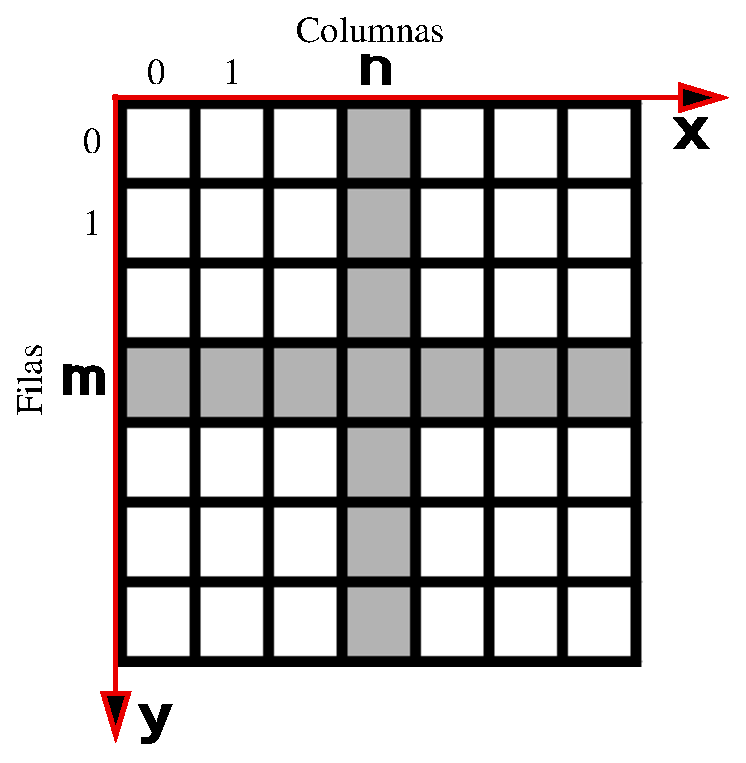
\includegraphics[width=0.5\textwidth]{Contenido/Cuerpo/Capitulo2/Fig8.eps}
	\captionof{figure}{Representación 2D de imágenes digitales mediante conjuntos de puntos discretos en una matriz rectangular}
	\label{fig:MarcoTeorico:Fig17}
\end{center}
La función de imagen f(x,y) es digitalizada en la memoria del computador, tanto
espacialmente como en amplitud. La digitalización de las coordenadas espaciales (x,y)
está asociada al concepto de muestreo, mientras que la digitalización de la amplitud al
de cuantificación de los niveles de gris.\cite{Book:Jose2005}
\\El muestreo es la conversión que sufren las dos dimensiones espaciales de la
señal analógica, y que genera la noción de píxel.\\
Los puntos 2D (coordenadas de píxeles en una imagen) se pueden denotar usando un par de valores, $x = (x,y) \in$ ${\textbf{I\!R}^2}$\cite{Book:Richard2011}
\begin{equation}
	x = \left[
		\begin{array}{c}
			x \\
			y
		\end{array}
		\right]
\end{equation}
Los puntos 2D también se pueden representar utilizando coordenadas homogéneas, $\tilde{x} = (\tilde{x},\tilde{y}, \tilde{w}) \in {\textbf{I\!P}^2}$
donde los vectores que difieren solo por escala se consideran equivalentes. ${\textbf{I\!P}^2} = {\textbf{I\!R}^3} -  (0,0,0) $ se llama el espacio proyectivo 2D.

% ----------------------------------------------------------------------------------------------------------------------------
% NUEVA SUBSECCION
% ----------------------------------------------------------------------------------------------------------------------------

\subsection{Cuantización}
Para usar con una computadora, la energía medida en el plano de la imagen debe
asignarse a un número limitado Q de valores discretos de gris. Este proceso se llama
cuantización. El número de niveles de cuantificación requeridos en el procesamiento de
imágenes se puede discutir con respecto a dos criterios.\cite{Book:Richard2011}\\
La cuantificación es la conversión
que sufre la amplitud de la señal analógica; así se genera el concepto de nivel de gris o
intensidad.En general, los datos de imagen se cuantifican en 256 valores de gris.
Luego, cada píxel ocupa 8 bits o un byte. Para el caso de tener 256 niveles de gris (0-255), el 0 corresponde a un
objeto no iluminado o que absorbe todos los rayos luminosos que inciden sobre él
(negro), y el nivel 255 a un objeto muy iluminado o que refleja todos los rayos que
inciden sobre él (blanco).
\begin{center}
	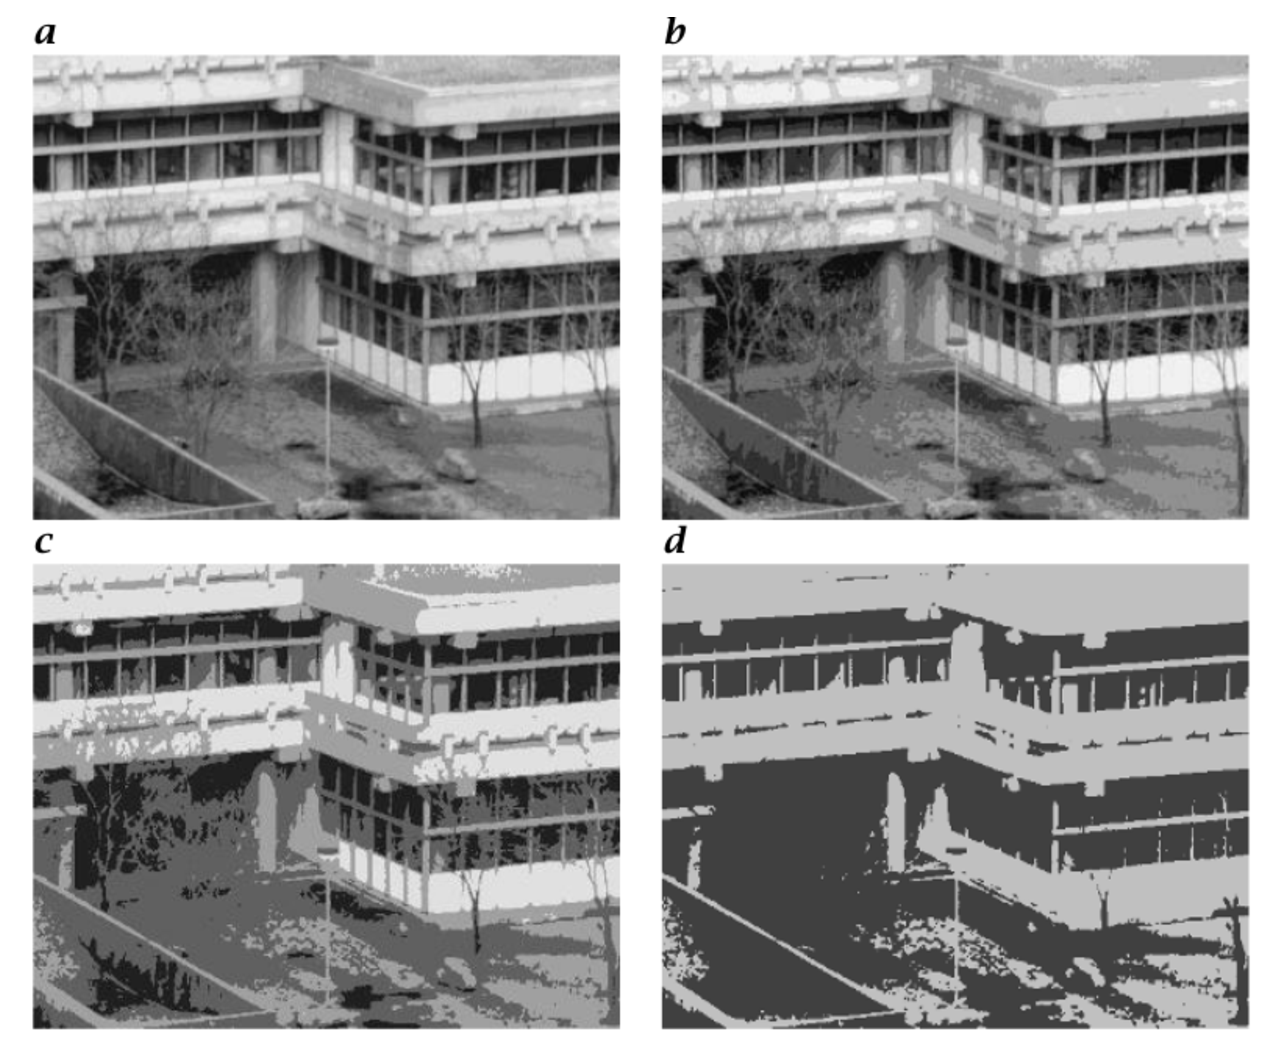
\includegraphics[width=0.6\textwidth]{Contenido/Cuerpo/Capitulo2/Fig9.eps}
	\captionof{figure}{Ilustración de cuantización\cite{Book:Bernd1997}.La misma imagen se muestra con diferentes niveles de cuantización: a 16, b 8, c 4, d 2. Muy pocos niveles de
		cuantificación producen bordes falsos y hacen que las características con bajo contraste desaparezcan parcial o totalmente.}
	\label{fig:MarcoTeorico:Fig18}
\end{center}
Al efecto de disminuir la resolución y mantener las
dimensiones físicas se le conoce como efecto tablero de ajedrez.

% ----------------------------------------------------------------------------------------------------------------------------
% NUEVA SUBSECCION
% ----------------------------------------------------------------------------------------------------------------------------
\subsection{Librerias OPENCV}
Dentro del mundo del procesamiento de imágenes digitales encontramos una amplia variedad
de desarrolladores que han construido librería especializadas en el tratamiento de
imágenes. Dentro de las que destacan nombres como OpenCV, HALCON, y point cloud library.
Siendo la primera de estas de código abierto. Por esta razón he decidido utilizar
OpenCV en este proyecto, aunado a que tiene soporte de contribuidores en todo el mundo.\\
OpenCV es una biblioteca open-source de Visión Artificial originalmente desarrollada por
Intel en 1999. Desde entonces se ha utilizado en infinidad de aplicaciones, desde
sistemas de seguridad con detección de movimiento, hasta aplicativos de control de
procesos donde se requiere reconocimiento de objetos. Contiene más de 500 funciones
que abarcan una gran gama de áreas en el proceso de Visión, como reconocimiento de
objetos, reconocimiento facial, calibración de cámaras, visión estéreo y visión
robótica y no dejan de añadirse nuevos algoritmos continuamente. Su principal ventaja
es que se puede utilizar de manera gratuita, incluso para realizar aplicaciones
comerciales.\cite{WEB:Opencv}
\begin{center}
	
\includegraphics[width=0.6\textwidth]{Contenido/Cuerpo/Capitulo2/Fig12.eps}
	\captionof{figure}{Símbolo característico RGB de OpenCV}
	\label{fig:MarcoTeorico:Fig19}
\end{center}
Tiene interfaces C ++, Python, Java y MATLAB y es compatible con Windows, Linux,
Android y Mac OS.

% ----------------------------------------------------------------------------------------------------------------------------
% NUEVA SUBSECCION
% ----------------------------------------------------------------------------------------------------------------------------
\subsection{Calibración de camara}
La calibración de cámaras es un paso esencial en la obtención de buenos resultados
el los algoritmos de visión artificial, dado su importancia es que hay múltiples
algoritmos que satisfacen la necesidad de tener una imagen clara y calibrada.\\
Cada uno estos algoritmos está destinado a ciertas características ópticas de nuestra
cámara.\\
Las cámaras han existido por mucho, mucho tiempo. Sin embargo, con la introducción de
las cámaras baratas de modelo pinhole a fines del siglo XX, se convirtieron en una
ocurrencia común en nuestra vida cotidiana. Desafortunadamente, este ahorro economico viene
con su precio: distorsión significativa. Afortunadamente, estas son constantes y con
una calibración y algunas reasignaciones podemos corregir esto. Además,
con la calibración también puede determinar la relación entre las unidades naturales
de la cámara (píxeles) y las unidades del mundo real (por ejemplo, milímetros).\cite{WEB:OpencvCalibracion}\\
En este proyecto abordaremos el método de calibración hecho por Zhang (Zhang, 1998, 2000)
que básicamente consiste en utilizar una plantilla 2D y que toma ventaja el hecho de tomar
calibración basadas en las medidas de
las coordenadas de la plantilla con las ventajas de la
auto calibración en la cual no es necesaria utilizar
plantilla.
% ----------------------------------------------------------------------------------------------------------------------------
% NUEVA SUBSECCION
% ----------------------------------------------------------------------------------------------------------------------------
\subsubsection{Espacio de color}
El uso del color en el procesamiento de imágenes está motivado por dos factores principales.
Primero, el color es un poderoso descriptor que a menudo simplifica la identificación y
extracción de objetos de una escena. En segundo lugar, los humanos pueden discernir miles
de tonos e intensidades de color, en comparación con solo los tonos de gris de una cámara.\cite{Book:Rafael2002}\\
El espacio de color es un espacio geométrico tridimensional con ejes adecuadamente
definidos para que los símbolos de todas las percepciones de color posibles de humanos u
otros animales encajen en él en un orden correspondiente al orden psicológico.
Los parámetros síquicos de la percepción del color son la luminosidad, el tono, y
la saturación. El propósito de un modelo de color (también llamado espacio de color) es
facilitar la especificación de colores de alguna manera estándar, generalmente aceptada.
En esencia, un modelo de color es una especificación de un sistema de coordenadas y un
subespacio dentro de ese sistema donde cada color está representado por un solo punto.\\
Hay multiples espacios de color en la actualida, siendo el espacio RGB el mas conocido, esto
debido a su antigua creación hecha por Helmholtz y Schrödinger, asumiendo
tres procesos fundamentales de visión del color R, G y B (Rojo, Verde y Azul).
\begin{equation}
	\frac{dR}{R} = \frac{dG}{G} = \frac{dB}{B} = constante
\end{equation}
donde dR es el incremento / decremento en magnitud del estímulo descrito por el proceso
fundamental R, y comparable para los otros dos estímulos.\cite{Book:Rolf2003}
\begin{center}
	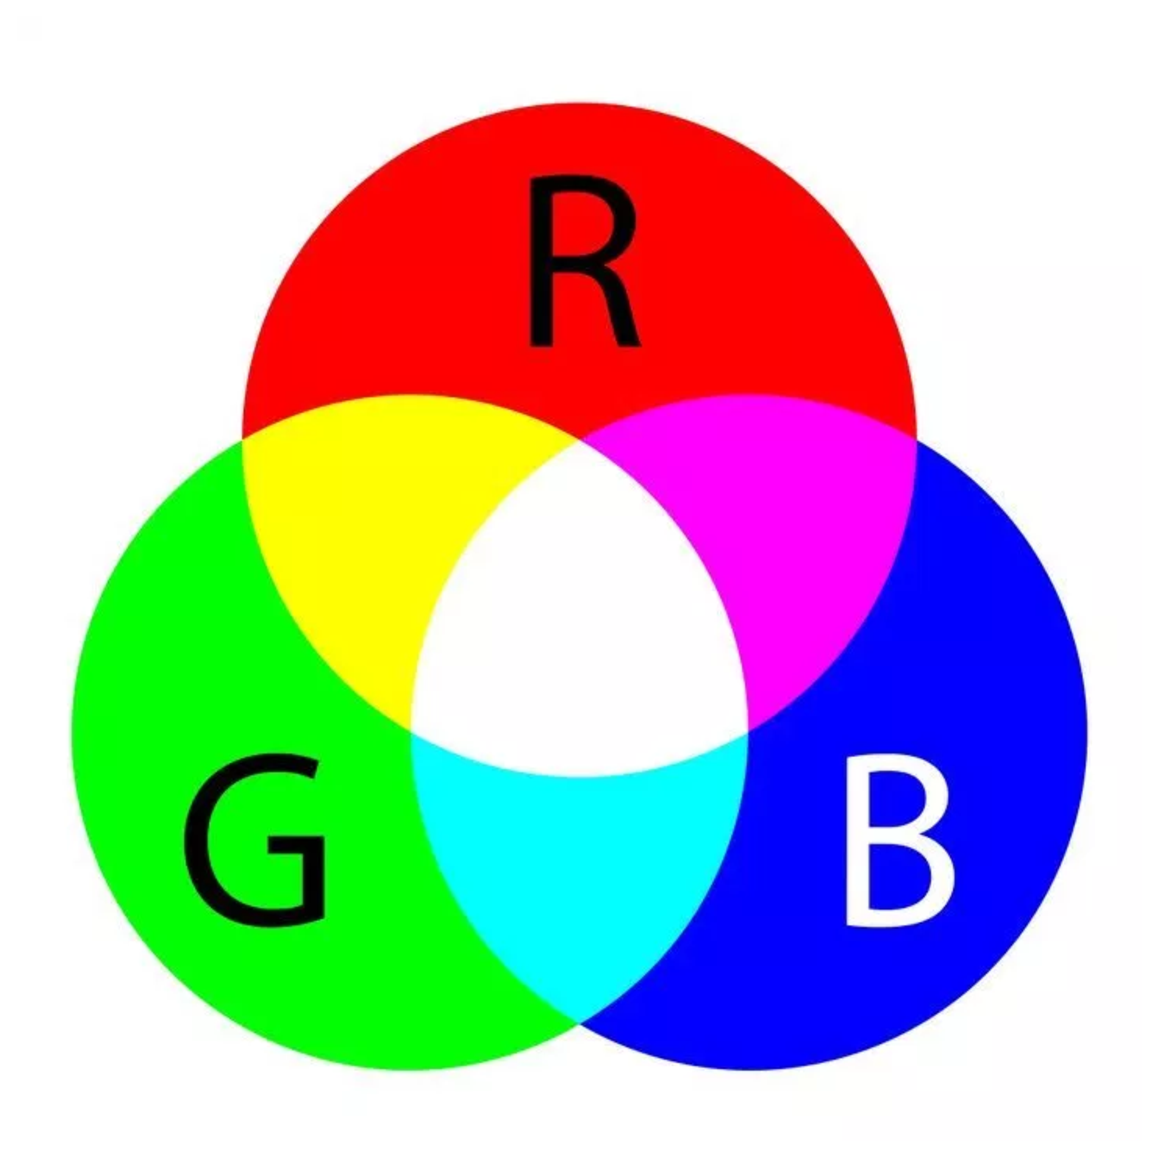
\includegraphics[width=0.35\textwidth]{Contenido/Cuerpo/Capitulo2/Fig10.eps}
	\captionof{figure}{Representación del espacio de color RGB}
	\label{fig:MarcoTeorico:Fig20}
\end{center}
Uno de los principales problema que el modelo RGB presenta es la mezcla de la información
del color (tono y saturación) y la intensidad. Aun así sigue siendo el modelo más utilizado y
el que los productores de cámara utilizan para ser implementadas en estas. Estos dos inconvenientes
se resuelven con el siguiente espacio de color.
\subsubsection{HSI}
"HSI" se refiere al modelo de color de Tono, Saturación, Intensidad para presentar datos
de color. El modelo de color de intensidad de saturación de tono (HSI) se parece mucho
a las propiedades de detección de color de la visión humana. El componente de intensidad
está relacionado con el componente de luminancia desacoplado del color. Los componentes
de matiz y saturación están relacionados con la forma en que un humano percibe el color.
Dicha relación con la visión humana hace que sea deseable utilizar el modelo de color
HSI para las técnicas de procesamiento de imágenes en color, como la mejora de imágenes
y la segmentación de imágenes.\cite{Article:taiy2000}\\
Las transformaciones matemáticas que permiten el paso del espacio RGB al HSI
son realizadas normalmente mediante hardware específico. Las ecuaciones son:
\begin{equation}
	I=\frac{R+G+B}{3}
\end{equation}
\begin{equation}
	H = arctan \left( \frac{\sqrt{3}(G-B)}{(R-G)+(R-B)} \right)
\end{equation}
\begin{equation}
	S = 1 - \frac{min(R,G,B)}{I}
\end{equation}
Así como el espacio RGB se representa por un cubo, el HSI lo forman dos
pirámides unidas por su base. Dependiendo de la intensidad se tiene un corte a los
conos.
\begin{center}
	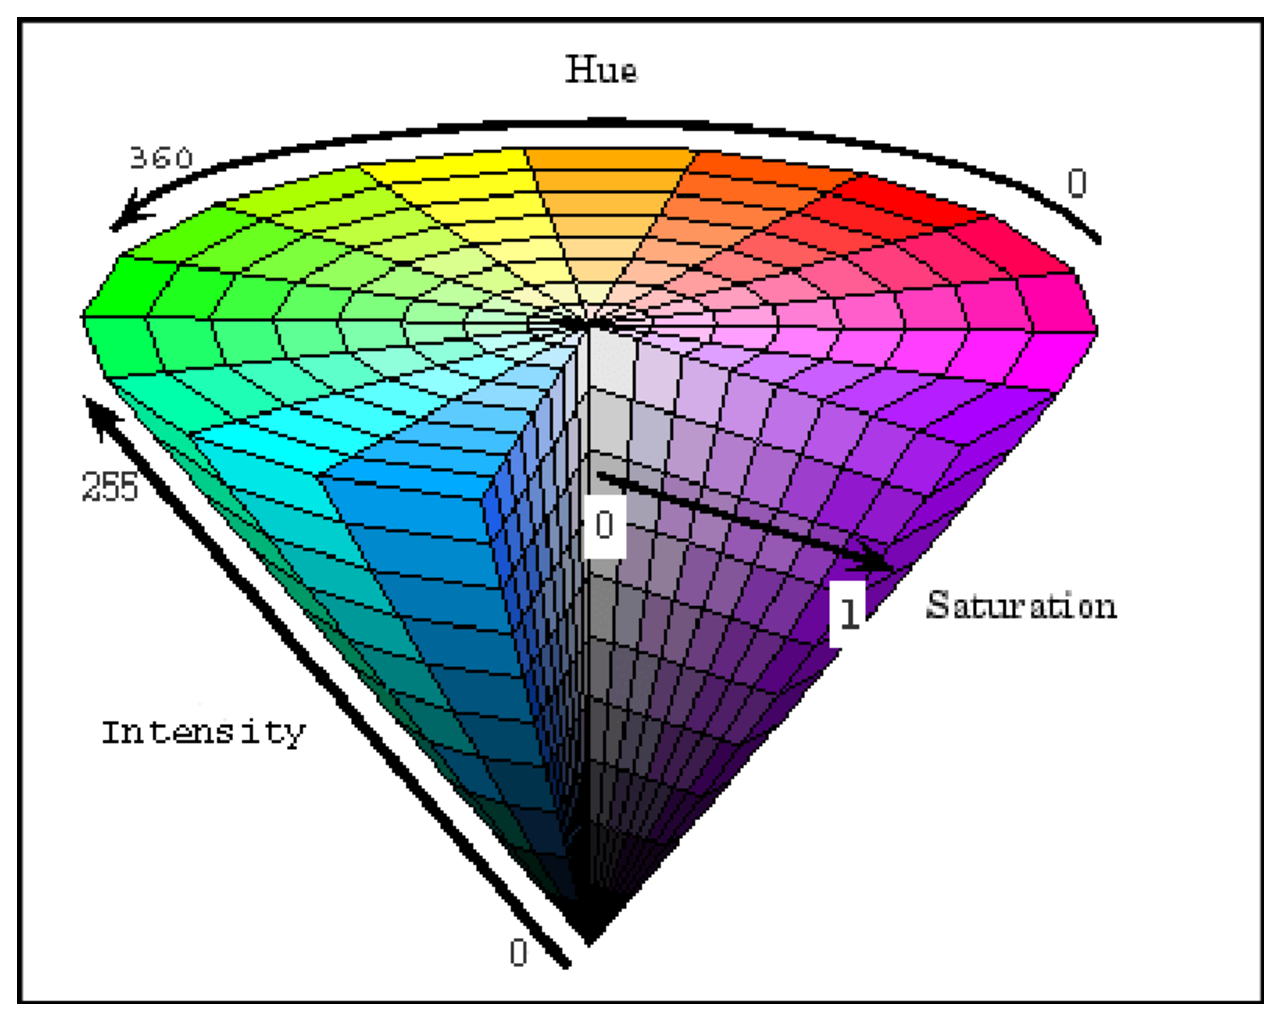
\includegraphics[width=0.5\textwidth]{Contenido/Cuerpo/Capitulo2/Fig11.eps}
	\captionof{figure}{Representación del espacio de color HSI}
	\label{fig:MarcoTeorico:Fig21}
\end{center}
Variaciones de este espacio de color son:
\begin{itemize}
	\item \textbf{HSL}(Hue, Saturation Lightness)
	\item \textbf{HSV} (Hue Saturation Value)
	\item \textbf{HCI} (Hue Chroma / Colourfulness Lightness)
	\item \textbf{HVC} (Hue Value Chroma)
	\item \textbf{TSD} (Hue Saturation Darkness)
\end{itemize}

\subsubsection{Características del modeldo HSV}
Esta variación del modelo HSI es la base en librerias dedicadas a la visión artificial,
En resumen tenemos los siguiente valores para cada característica de este modelo.\\
\textbf{Tono(H)}\\
El tono es la porción de color del modelo, expresada como un número de 0 a 360 grados:
\begin{itemize}
	\item El rojo cae entre 0 y 60 grados.
	\item El amarillo cae entre 61 y 120 grados.
	\item El verde cae entre 121-180 grados.
	\item El cian cae entre 181-240 grados.
	\item El azul cae entre 241-300 grados.
	\item Magenta cae entre 301-360 grados.
\end{itemize}
\textbf{Saturación}\\
La saturación describe la cantidad de gris en un color particular, del 0 al 100 por
ciento. La reducción de este componente hacia cero introduce más gris y produce un
efecto desvanecido. A veces, la saturación aparece como un rango de solo 0-1, donde 0
es gris y 1 es un color primario.\\
\textbf{Valor(V)[brillo]}\\
El valor funciona junto con la saturación y describe el brillo o la intensidad del
color, de 0 a 100 por ciento, donde 0 es completamente negro y 100 es el más brillante
y revela la mayor cantidad de color.

\subsubsection{Espacio de color en OpenCV}
En el caso de imágenes de 8 bits y 16 bits, R, G y B se convierten al formato
de punto flotante y se escalan para ajustarse al rango de 0 a 1.
\begin{equation}
	V \leftarrow max(R,G,B)
\end{equation}
\begin{equation}
	S \leftarrow \begin{cases} \frac{V-min(R,G,B)}{V}, & \mbox{if } V\mbox{ = R} \\ 0, & \mbox{otherwise }  \end{cases}
\end{equation}
\begin{equation}
	H \leftarrow \begin{cases}
		60(G - B)/(V-min(R,G,B)),           & \mbox{if } V\mbox{ = R} \\
		{{120+60(B - R)}/{(V-min(R,G,B))}}, & \mbox{if } V\mbox{ = G} \\
		{{240+60(R - G)}/{(V-min(R,G,B))}}, & \mbox{if } V\mbox{ = B} \\
	\end{cases}
\end{equation}
Si $H < 0$ entonces $H \leftarrow H+360$. En la salida tenemos $0 \leq V \leq 1$,
$0 \leq S \leq 1$ , $0 \leq H \leq 360$.
Los valores se convierten luego al tipo de datos de destino:
\begin{itemize}
	\item Imagen de 8 bits: $V \leftarrow 255V$, $S\leftarrow 255S$, $H \leftarrow H/2$(para ajustar de 0 a 255)
	\item Imágenes de 16 bits: (actualmente no compatible)
	\item Imágenes de 32 bits: H, S y V se dejan como están
\end{itemize}
\cite{WEB:Opencvcolor}

% ----------------------------------------------------------------------------------------------------------------------------
% NUEVA SUBSECCION
% ----------------------------------------------------------------------------------------------------------------------------

\subsection{Transformaciones morfológicas}
Lo que conocemos como realidad proviene de las percepciones obtenidas por los sentidos, por ejemplo el sentido de la vista
nos puede entregar un objeto casi que borroso pero nuestra memoria y capacidad de asociamiento nos permite relacionarlo con
algún objeto guardado en nuestra base de datos.\\
Hacer lo anterior en un sistema embebido involucra tener una base de datos amplio, lo que genera un costo razonable de recursos
de memoria y procesamiento, debido a esto es que existen diversas maneras de "limpiar" lo que nuestros sentidos captan, que en
este caso es lo que capta la cámara, tengan el menor ruido posible.\\
Es aquí donde las transformaciones morfológicas toman lugar, debido a su uso en imágenes binarias que permiten simplificar
el uso de imágenes digitales. Estas basan su funcionamiento en una rama de las matemáticas conocidas como "Teoría de conjuntos".
Se puede consultar más información acerca de la matemática detrás de las operaciones morfológicas y teoría de conjuntos en la
obra de \cite{Book:Serra1984} %\cite{Serra1984} \\ 
\subsubsection{Conceptos elementales de teoría de conjuntos}
Algunas definiciones básicas son descritas, tomando en cuenta que la notación para estos son mayúsculas (X, Y, Z \dots), mientras
que para los elementos son las minúsculas (q, r, t \dots).\\
Las siguientes definiciones fueron tomadas de \cite{10045_10053}
\theoremstyle{definition}
\begin{definition}{\textbf{Inclusión}}
	X es subconjunto de Y si todos los elementos de X pertenecen a Y:
	\begin{equation}
		X \subseteq Y 	\iff \{ p \in X \rightarrow p \in Y \}
	\end{equation}
	La inclusión es reflexiva, antisimétrica y transitiva.
\end{definition}
\begin{definition}{\textbf{Complemento}}
	El complemento de X, $X^c$, son todos los elementos que no pertenecen a X.
\end{definition}
\begin{definition}{\textbf{Unión}}
	La unión de dos conjuntos se constituye por los elementos que pertenecen a uno o al otro:
	\begin{equation}
		X \cup Y = \{ p|p \in X \quad o  \quad p \in Y \}
	\end{equation}
	Al igual que la intersección, la unión de conjuntos es conmutativa, asociativa e idempotente
\end{definition}
\begin{definition}{\textbf{Intersección}}
	La intersección de dos conjuntos X e Y es el conjunto de los elementos que pertenecen a ambos conjuntos:
	\begin{equation}
		X \cap Y = \{ p|p \in X \quad y \quad p \in Y \}
	\end{equation}
	La intersección es conmutativa, asociativa e idempotente. Esta última propiedad es importante en morfología y
	significa que $X \cap X = X$.
\end{definition}
\begin{definition}{\textbf{Translación}}
	Un conjunto X es trasladado por un vector $v$, cuando cada uno de los elementos de ese conjunto sufre esa translación.
	Se denominará al nuevo conjunto $X_v$.
\end{definition}

\subsubsection{Transformaciones morfológicas elementales}
Las transformaciones morfológicas son algunas operaciones simples basadas en la forma de la imagen. Normalmente se realiza en
imágenes binarias.Necesita dos entradas, una es nuestra imagen original, la segunda se llama elemento de estructuración o
kernel que decide la naturaleza de la operación.Dos operadores morfológicos básicos son la erosión y la dilatación. Luego,
sus variantes de formas como Apertura, Cierre, Gradiente, etc. también entran en juego. \cite{WEB:Ieeeucsa2019}\\
Para el presente trabajo, todas las entradas son imágenes binarias, esto es, blanco y negro provenientes de la salida
del proceso del cambio de espacio de color a HSV, donde el color blanco representa el segmento del objeto a seguir.Además de que
las operaciones morfológicas serán aplicadas como filtros de ruido en la imagen, debido a eso solo serán necesarias dos operaciones:
apertura y cierre, que están basadas en erosión y dilatación.\\
La esencia de las transformaciones morfológicas es la obtención de estructuras geométricas en los conjuntos donde sé está procesando,
mediante el empleo de otro conjunto de forma conocida, a este último se le denomina como elemento estructurante.
El tamaño y la forma del elemento estructurante se selecciona de acuerdo a las formas que el usuario requiera obtener.
\begin{center}
	
\includegraphics[width=0.4\textwidth]{Contenido/Cuerpo/Capitulo2/Fig13.eps}
	\captionof{figure}{ Ejemplo de formas básicas de elementos estructurantes planos}
	\label{fig:MarcoTeorico:Fig22}
\end{center}


\subsubsection{Erosión}
La transformación de erosión es el resultado de comprobar si el elemento estructurante
Y está totalmente incluido dentro del conjunto X. Cuando esto no ocurre, el resultado de la
erosión es el conjunto vacío. \cite{10045_10053}.\\
La erosión de un conjunto X por un elemento estructurante Y se define como el conjunto
de puntos o elementos x, pertenecientes a X, de forma que cuando el elemento estructurante Y se
traslada a ese punto, el elemento queda incluido en X. \cite{10045_10053}.\\
Entonces podemos definir matemáticamente a la erosión de la siguiente manera:
\begin{equation}
	X \Theta \tilde{B} = \{ x|B_x \subset X \}
\end{equation}
de donde
\begin{itemize}
	\item $\Theta$ = Resta de Minkowski
	\item $\tilde{B}$ = Elemento estructural simetrico
\end{itemize}
Que en palabras del autor de la obra \cite{Book:Arturo2011} la erosión es la degradación progresiva de uno de los campos (0 ó 1). Un elemento del
campo a degradar seguirá perteneciendo al mismo si está rodeado de elementos iguales
a él. En caso contrario, pasará al otro campo. En un proceso iterativo terminaría por
destruir la imagen.\\
De la ecuación 2.17 podemos decir entonces que la erosión es más pronunciada con base en el tamaño del elemento estructural.
\begin{center}
	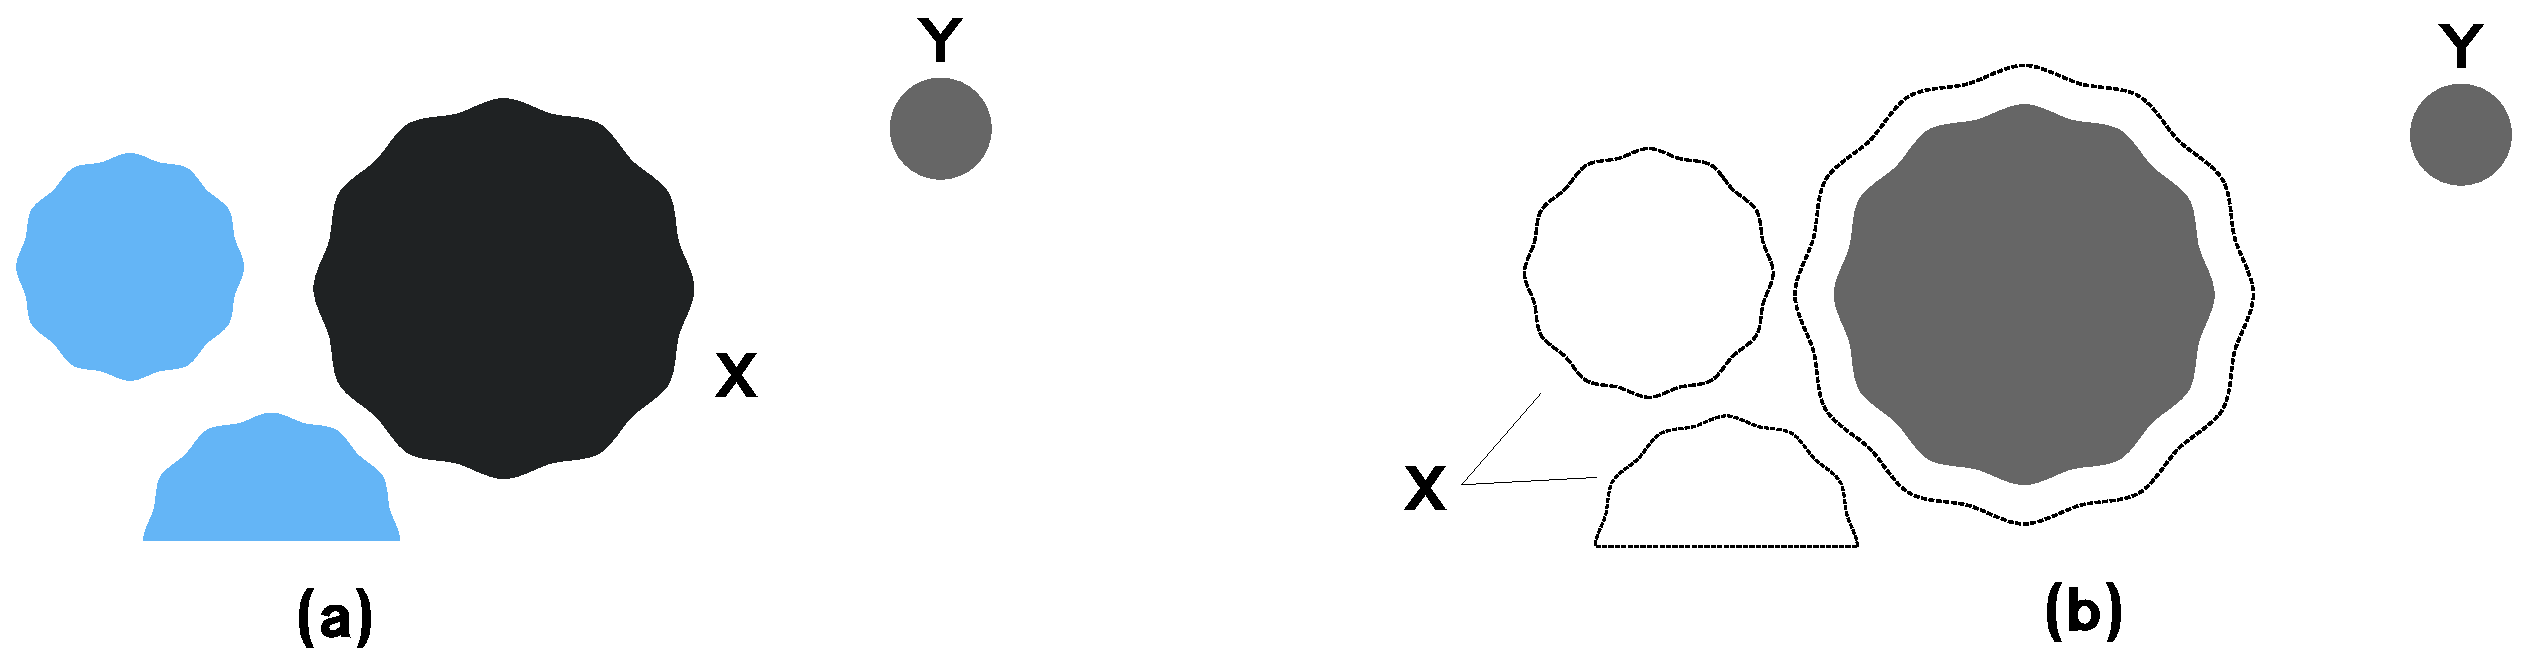
\includegraphics[width=0.8\textwidth]{Contenido/Cuerpo/Capitulo2/Fig14.eps}
	\captionof{figure}{(a) Erosión de X por el elemento estructurante Y. (b) Los elementos conectados del conjunto X más pequeños que Y son eliminados. }
	\label{fig:MarcoTeorico:Fig23}
\end{center}
De la imagen anterior se puede observar como en (b) el proceso de erosión disminuye la dimensión de las figuras, y en algunos casos elimina la totalidad de estos.

\subsubsection{Dilatación}
La transformación de dilatación es el proceso "inverso" al de la erosión, en otras palabras, las operaciones de erosión y dilatación son duales una de otra.\\
Es el crecimiento progresivo de uno de los campos (0 ó 1). Un elemento del
campo contrario a crecer será convertido si posee algún vecino perteneciente al campo
que se expansiona. En caso contrario, permanecerá igual. Los elementos pertenecientes
al campo a expansionar evidentemente no se modifican.\cite{Book:Jose2005}\\
Tomando en cuenta la dualidad antes mencionada, podemos obtener matemáticamente la dilatación de la siguiente manera:
\begin{equation}
	X \otimes \tilde{B} = (X^c \otimes \tilde{B})^c
\end{equation}
La siguiente figura ilustra el resultado de aplicar la operación de dilatación de donde el elemnto estructurante Y tiene forma de disco.
\begin{center}
	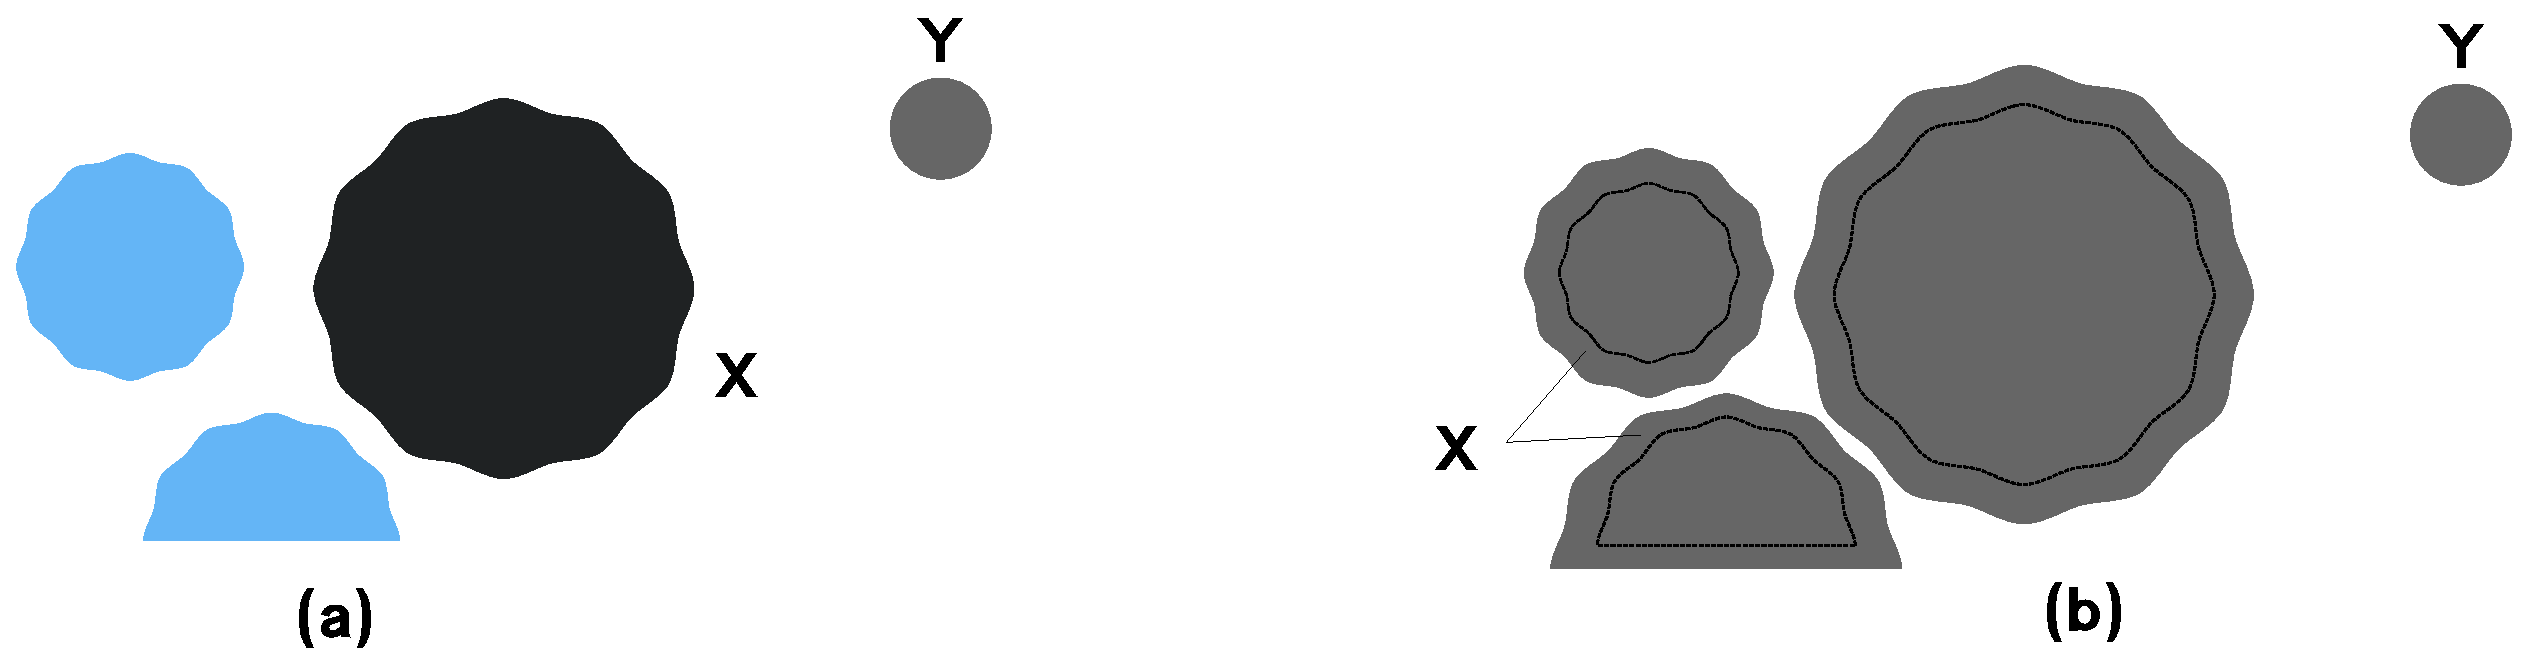
\includegraphics[width=0.8\textwidth]{Contenido/Cuerpo/Capitulo2/Fig15.eps}
	\captionof{figure}{(a) Dilatación de X por el elemento estructurante Y. (b) El conjunto X aumenta su definición.  }
	\label{fig:MarcoTeorico:Fig23}
\end{center}
Como se puede observar en (b) el elemnto estructurante Y aumenta la definición del objeto X.

\subsubsection{Apertura y Cierre}
En términos de morfología básica, hay dos operaciones fundamentales que funcionan como filtros en imágenes digitales, estos son conocidos como apertura
y cierre. Una vez definido la dilatación como $X \rightarrow \delta(X)$ y la erosión como $X \rightarrow \epsilon(X)$ y conociendo el principio
básico de su funcionamiento podemos darnos cuenta que no hay manera de determinar el origen de X desde las imágenes $\delta(x)$ o $\epsilon(X)$
, es decir, que no admiten inversa, pero es posible aproximarse a la forma genuina de X mediante la aplicación de la operación de erosión
seguida de la dilatación, al proceso anterior se le conoce como apertura. Mientras que si efectuamos una dilatación seguida de una erosión se conoce
como cierre.

\subsubsection{Apertura}
La
apertura (opening en la literatura anglosajona) se definirá entonces como una
combinación de erosiones y dilataciones en las que lo primero es un erosión y la última
una dilatación, siempre con el mismo elemento estructural:\cite{Book:Jose2005}
\begin{equation}
	X \circ B = (X \Theta \tilde{B})
\end{equation}
\begin{center}
	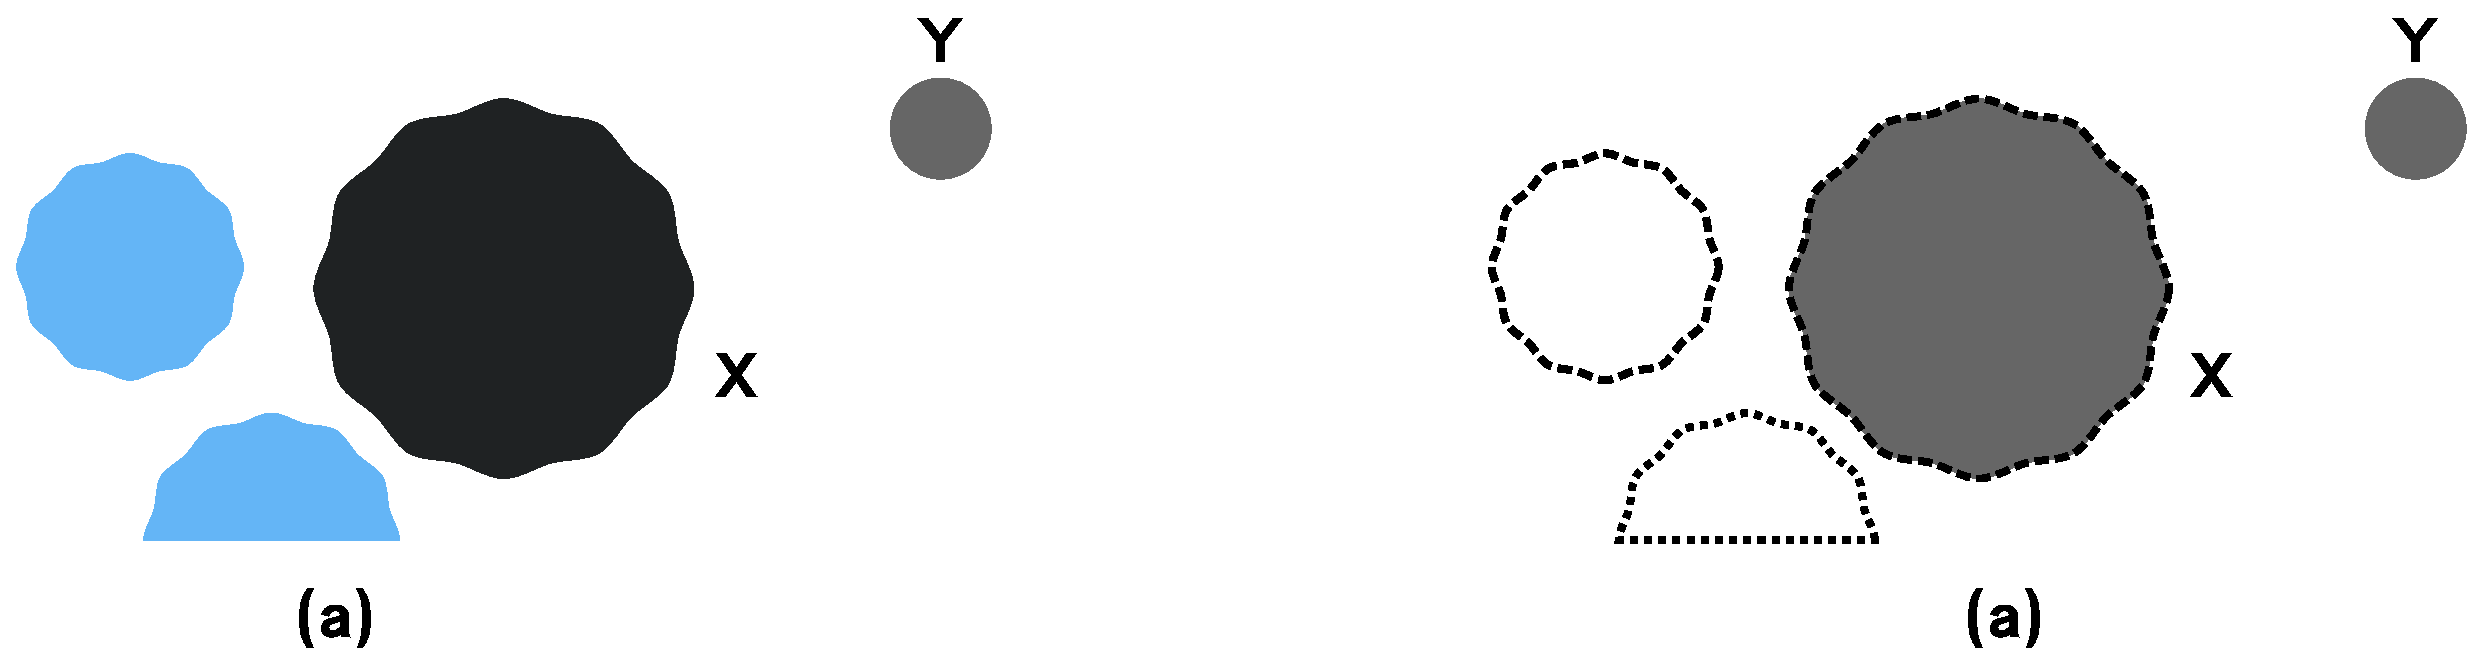
\includegraphics[width=0.8\textwidth]{Contenido/Cuerpo/Capitulo2/Fig16.eps}
	\captionof{figure}{(a) Apertura morfológica del conjunto X por el elemento estructurante Y. (b) Eliminación de objetos
		menores en tamaño al elemento estructurante. La apertura redondea las convexidades importantes.   }
	\label{fig:MarcoTeorico:Fig24}
\end{center}

\subsubsection{Cierre}
La dualidad de la operación de apertura es la del cierre(closing en literatura anglosajona), asi que podemos definirlo matemáticamente asi:
\begin{equation}
	X  \bullet B = (X \odot \tilde{B}) \Theta B
\end{equation}

\begin{center}
	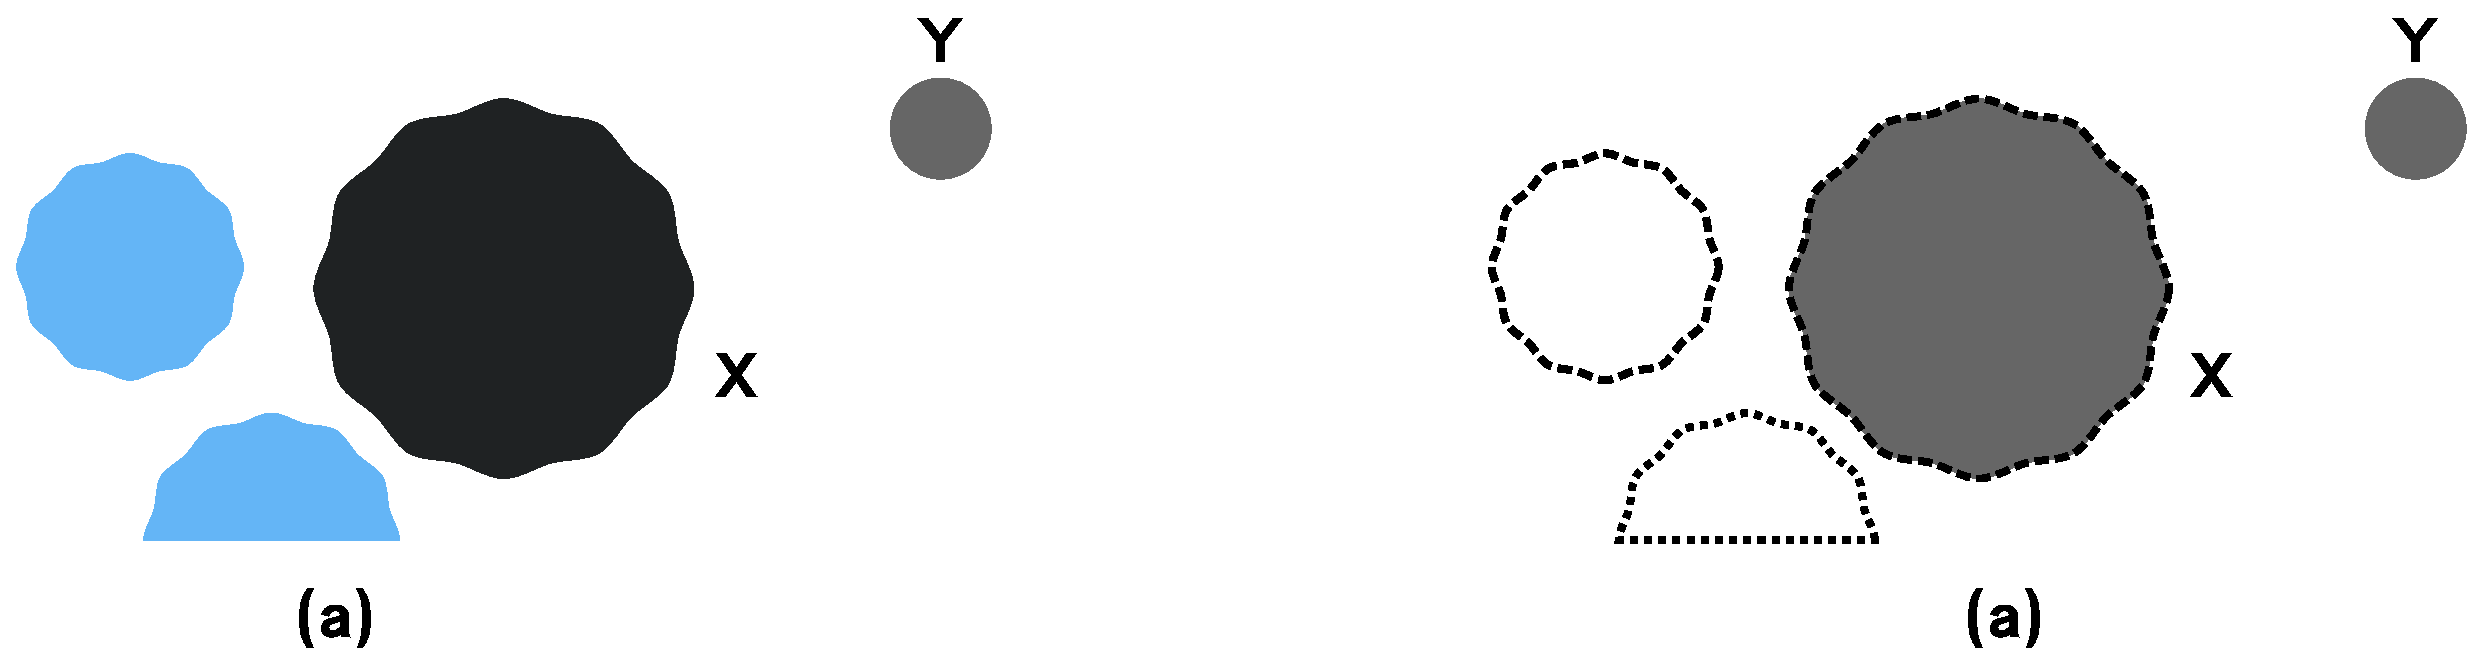
\includegraphics[width=0.8\textwidth]{Contenido/Cuerpo/Capitulo2/Fig16.eps}
	\captionof{figure}{(a) Apertura morfológica del conjunto X por el elemento estructurante Y. (b) El cierre redondea las
		concavidades importantes.    }
	\label{fig:MarcoTeorico:Fig25}
\end{center}

% ----------------------------------------------------------------------------------------------------------------------------
% NUEVA SUBSECCION
% ----------------------------------------------------------------------------------------------------------------------------

\subsection{Contraste y brillo}
Hablar de contraste y brillo es hablar de transformación de pixeles que a su vez hace referencia a otro termino que aún
no se ha abordado en este proyecto, que es el de operador de procesamiento de imagen. En la obra \cite{Book:Richard2011}
dicho operador es definido como:
\begin{equation}
	g(x) = h(f(x)) \quad o \quad g(x) = h(f_0(x) \dots f_n(x))
\end{equation}
Donde g(x) y h(x) son definidas como imagen.\\
Es decir que un operador es una imagen de salida tomando una o varias imágenes de entrada, que para un sistema discreto
la ecuación anterior se obtiene:
\begin{equation}
	g(i,j) = h(f(i,j))
\end{equation}
De donde i,j se acotan en las especificaciones del sensor de la cámara. \\Dos procesos puntuales de uso común
son la multiplicación y la suma con una constante,
\begin{equation}
	g(x) = \alpha f(x) + \beta
\end{equation}
\begin{itemize}
	\item El parámetro $\alpha$ > 0 es conocido como 'Gain' y es el encargado de controlar el nivel de contraste.
	\item El parámetro $\beta$ es conocido como 'Bias' y se encarga de controlar el brillo.
\end{itemize}
Y de igual manera que en la ecuación 2.22 podemos acotar la ecuacion 2.23 de la siguiente manera:
\begin{equation}
	g(i,j) = \alpha * f(i,j) + \beta
\end{equation}
Donde i, j nos indican la ubicación de los pixeles.

% ----------------------------------------------------------------------------------------------------------------------------
% NUEVA SUBSECCION
% ----------------------------------------------------------------------------------------------------------------------------
\subsection{Teorema de Green}
En el campo de las matemáticas hay un teorema que nos da la relación entre una integral
de línea, es decir donde la función a integrar se evalúa a lo largo de una curva, C y una
integral doble sobre una región plana D con límites C, tal como se ilustra en la siguiente
figura.
\begin{center}
	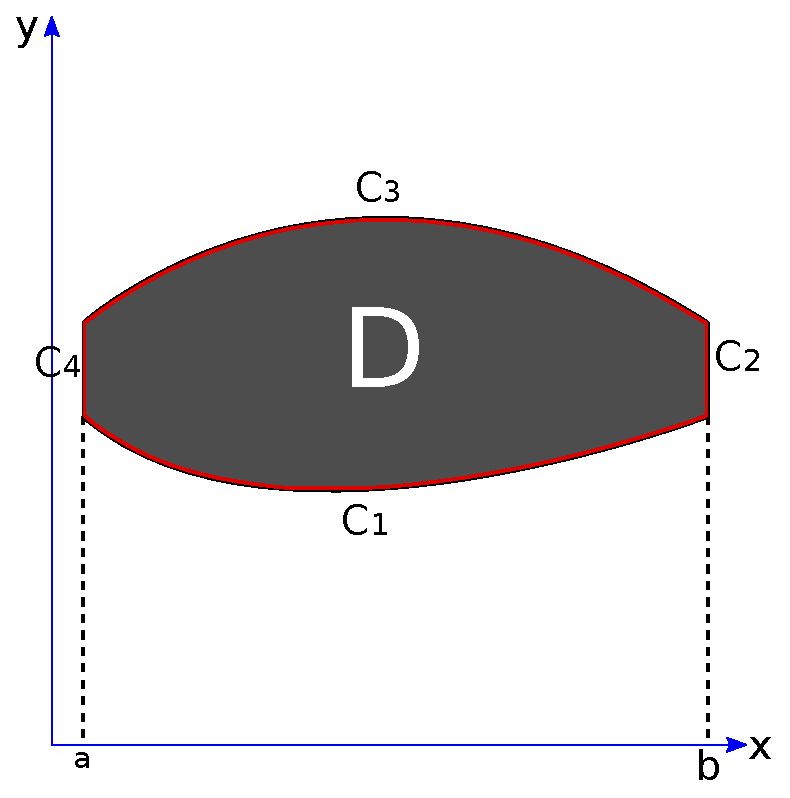
\includegraphics[width=0.4\textwidth]{Contenido/Cuerpo/Capitulo2/Fig18.eps}
	\captionof{figure}{Area de D limitada por C }
	\label{fig:MarcoTeorico:Fig25}
\end{center}
Dicho teorema es ampliamente utilizado para la detección de bordes. Si lo aterrizamos
en el campo de la visión artificial, y del trabajo de \cite{Paper::Lauren1994} podemos
obtener que el momento de orden (p + q) de una imagen bidimensional g (x, y) se define
como
\begin{equation}
	m_{pq} = \int_{y}^{} \int_{x}^{} g(x,y) x^p y^q dx dy
\end{equation}
Que para imagenes digitales tenemos entonces 
\begin{equation}
	m_{pq} = \sum_{y}^{}\sum_{x}^{} g(x,y) x^p y^q 
\end{equation}
Que de lo anterior y suponiendo que tenemos imagenes binarias, osea que 1 para objetos
y 0 para el fondo la ecuación queda asi
\begin{equation}
	m_{pq} = \sum_{(x,y)}^{}\sum_{\in R}^{}  x^p y^q 
\end{equation}
De donde R es la region del objeto.
\begin{definition}{\textbf{Momento}}
	El momento $M_{pq}^{(f)}$ de una imagen f(x,y), donde p,q son enteros positivos y r = p+q es
	el orden del momento.
	\begin{equation}
		M_{pq}^{(f)} = \int_{D}^{} \int_{}^{} p_{pq}(x,y) f(x.y) dxdy
	\end{equation}
	donde $p_{00}(x,y)$, $p_{10}(x,y)$, \dots, $p_{kj}(x,y)$ son funciones de base polinomiales 
	definidas en D.
\end{definition}

\subsubsection{Momentos}
La opción más común es una base de potencia estándar \cite{Book:Jan2009} $p_{kj}(x,y) = x^k y^j$
eso lleva a momentos geométricos. Que para imagenes binarias obtenemos lo siguiente
\begin{itemize}
	\item $m_{00}$ =  Es la 'masa' de la imagen, para imagenes binarias es el area del objeto.
	\item $m_{10}/m_{00}$ y $m_{01}/m_{00}$ = define el centro de gravedad, o en otras palabras
	el centroide de la imagen.
	\item $m_{20}$ y $m_{02}$ = Describen la 'distribución de masas' de la imagen con respecto a
	los ejes x,y
\end{itemize}
\chapter{Modelo matemático}
\cleanchapterquote{In mathematics, you don’t understand things. You just get used to them.}{John von Neumann}{(mathematician, physicist, computer scientist, and polymath.)}

En el presente capitulo se aborda el modelo matemático para el seguimiento de objetivos de una gimbal embebida en un UAV.

\section{Marco de referencia}
Los movimientos de la gimbal se basan en las coordenadas horizontales de azimuth y elevación, para gimbal de 3 grados de libertad
se agrega un tercer eje cuyo movimiento se conoce como roll. El eje de azimuth y la elevación se visualizan más fácilmente al
pensar en la posición de un objeto en relación con el horizonte.
\begin{center}
	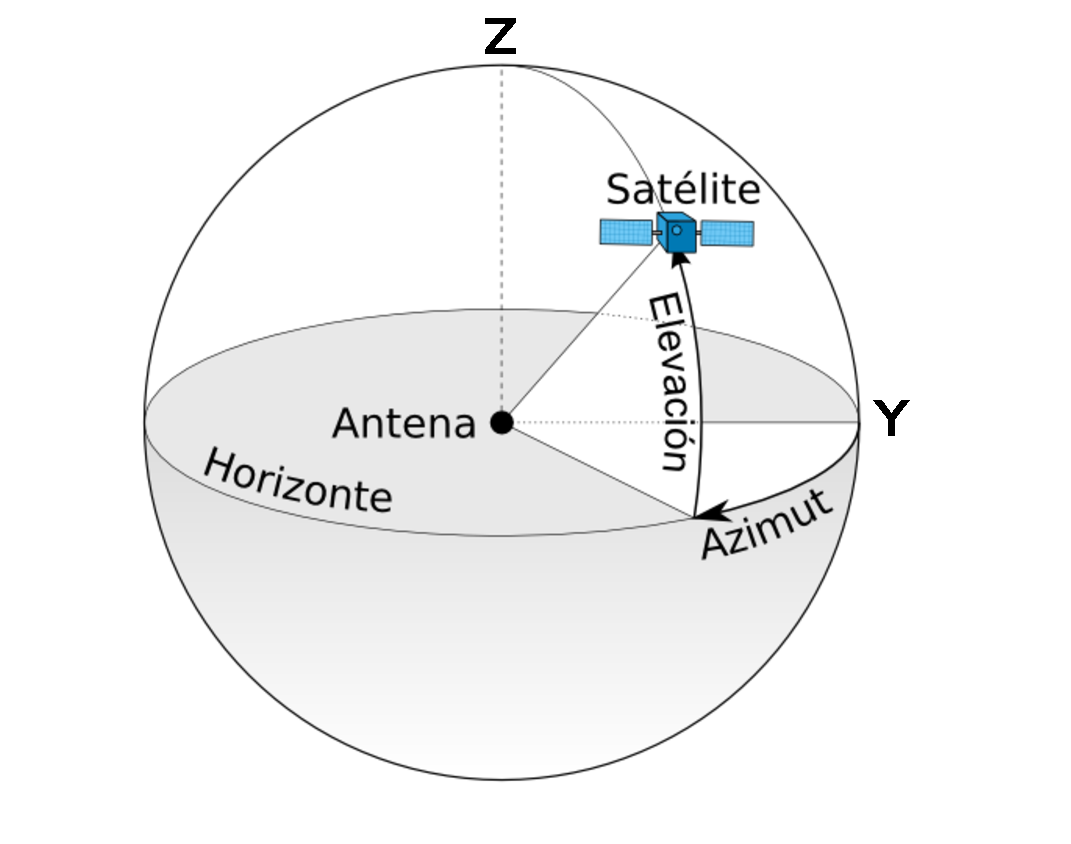
\includegraphics[width=0.55\textwidth]{Contenido/Cuerpo/Capitulo3/Fig1.eps}
	\captionof{figure}{Angulo de azimuth}
	\label{fig:ModeloMat:Fig1}
\end{center}
El angulo de azimuth es la posición alrededor del horizonte, medida desde un punto de referencia como el norte verdadero o el sur
verdadero. Los movimientos de azimuth ocurren alrededor del eje Z (vertical).

La elevación es la distancia del objeto por encima o por debajo del horizonte (también conocida como altitud en aplicaciones de
astronomía y aeroespaciales). Los movimientos de elevación ocurren alrededor del eje Y.

Los movimientos de balanceo ocurren alrededor del eje X a medida que gira con los ejes Y y Z.\\
El control que se hace en la gimbal está dado por un motor con control de posición y una IMU (sensor inercial).Dicha gimbal esta
montada en la parte delantera del vehículo aéreo como se muestra en la siguiente figura.
\begin{center}
	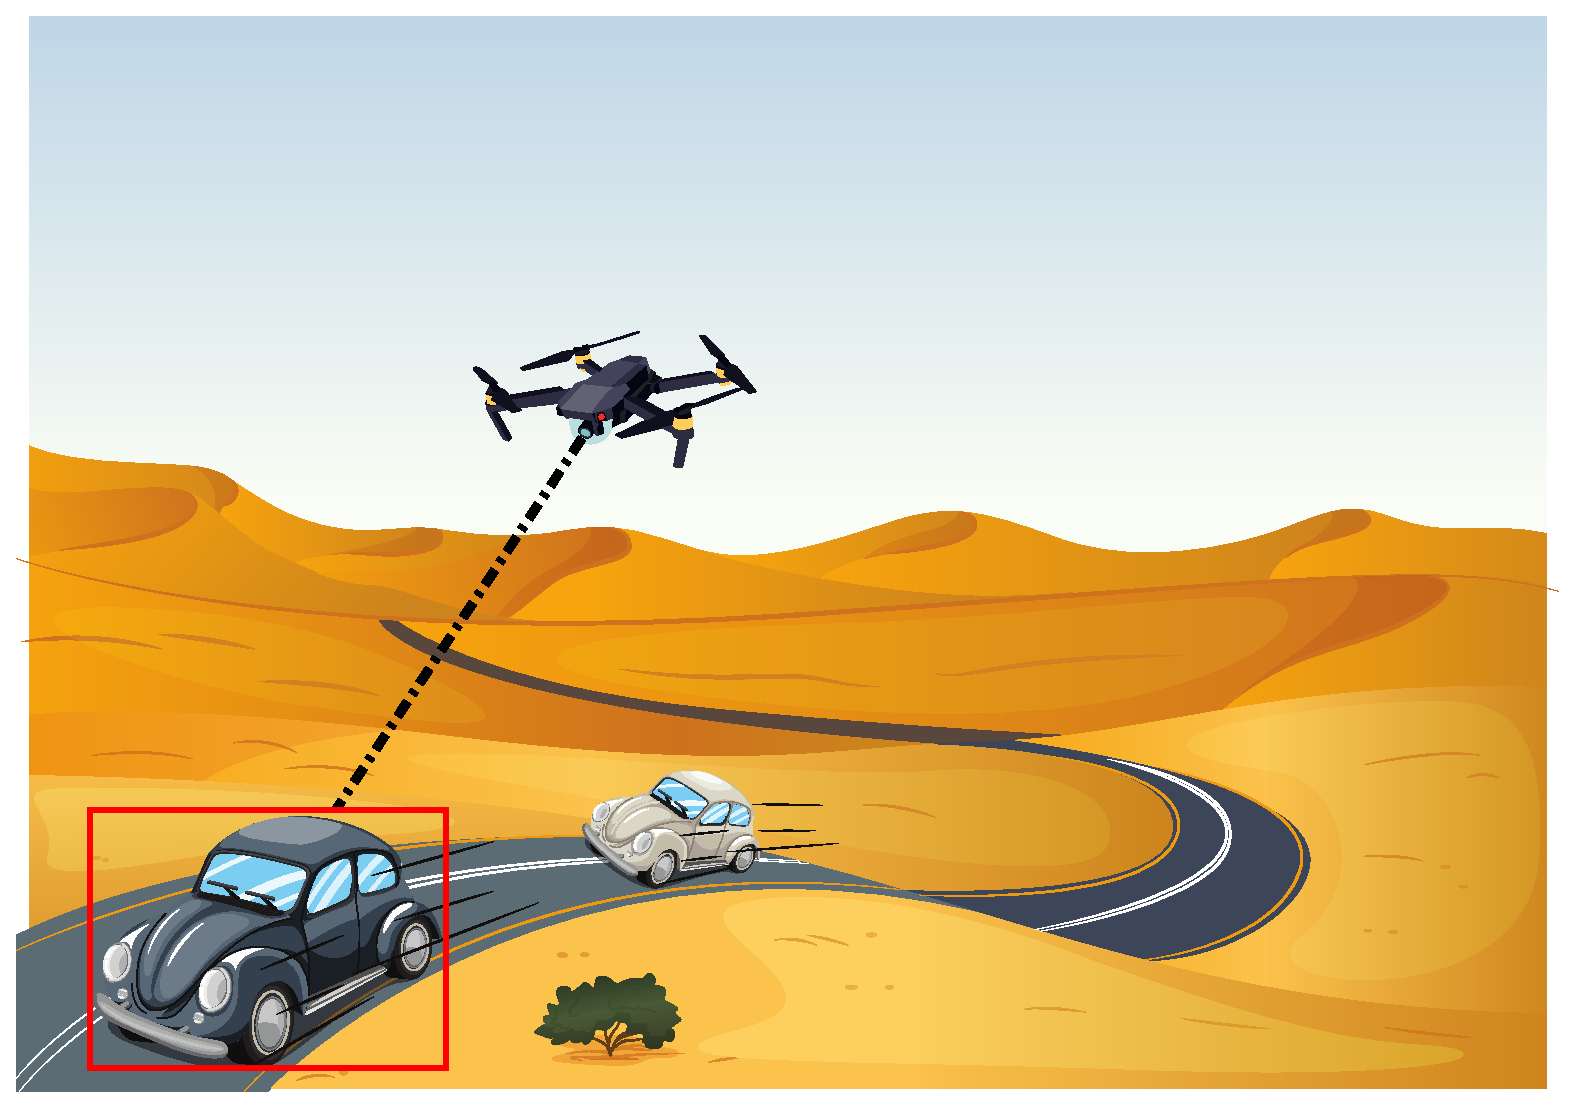
\includegraphics[width=0.55\textwidth]{Contenido/Cuerpo/Capitulo3/Fig2.eps}
	\captionof{figure}{Seguimiento de un objetivo utilizando una cámara sujeta a una gimbal embebida en un vehículo aéreo no tripulado.}
	\label{fig:ModeloMat:Fig1}
\end{center}

\subsection{Marco de referencia Inercial [I]}
Antes de abordar el control de la gimbal, es necesario y obvio conocer el comportamiento
de dicho sistema, empezaremos por definir el marco de referencia inercial, es decir
el de la tierra. La siguiente imagen ilustra los ejes de este marco.
\begin{center}
	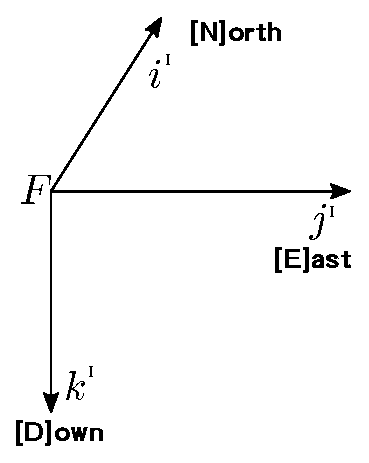
\includegraphics[width=0.25\textwidth]{Contenido/Cuerpo/Capitulo3/Fig4.eps}
	\captionof{figure}{Marco de referencia inercial}
	\label{fig:ModeloMat:Fig1}
\end{center}
Donde definimos a k apuntando hacia el centro de la tierra, este sistema de coordenadas
refieren a (Norte, Este y Abajo) de ahí su nombre NED(siglas en inglés).

\subsection{Marco de referencia del cuerpo [B]}
Una aeronave tiene la libertad de rotar en 3 ejes, en la aeronáutica son conocidos como
Yaw, Pitch y Roll. Dichas rotaciones son importantes en el control de aeronaves ya
que sirven para conocer la dinámica del sistema, dicha rotaciones pueden ser mejor
detalladas en una imagen, por lo que en la siguiente ilustración se grafica un plano
y se asigna nombre a cada rotación de los ejes.
\begin{center}
	
\includegraphics[width=0.35\textwidth]{Contenido/Cuerpo/Capitulo3/Fig6.eps}
	\captionof{figure}{Rotación en 3 ejes.}
	\label{fig:ModeloMat:Fig1}
\end{center}
Vamos a llamar marco de referencia del cuerpo a las coordenadas del UAV, es necesario establecer el centro del plano en el 
centro de masas de la aeronave, como se ilustra en la siguiente figura.
\begin{center}
	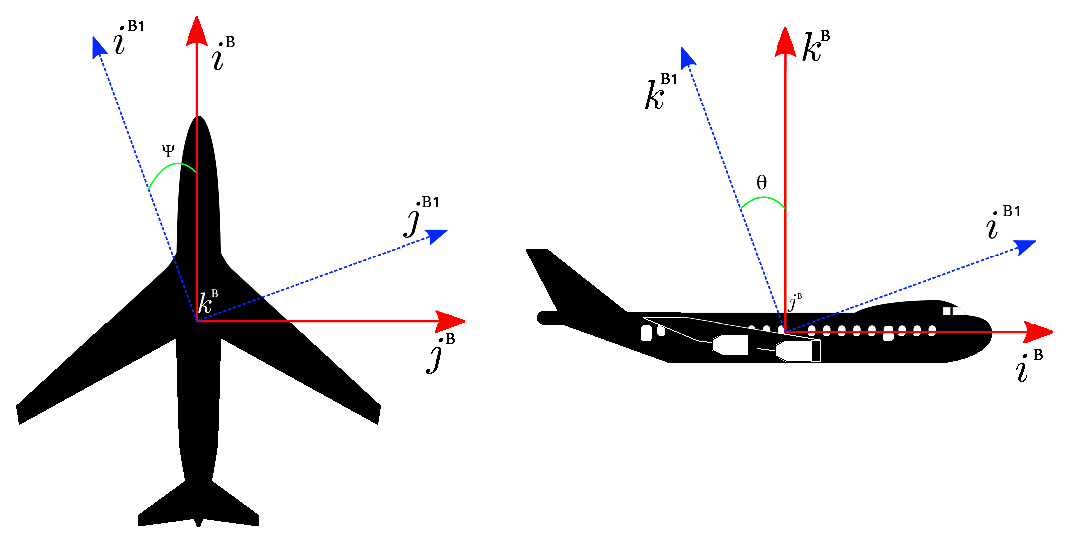
\includegraphics[width=0.5\textwidth]{Contenido/Cuerpo/Capitulo3/Fig5.eps}
	\captionof{figure}{Marco de referencia del cuerpo.}
	\label{fig:ModeloMat:Fig1}
\end{center}
De donde definimos las dos rotaciones que seran controladas en este trabajo pitch y yaw($\theta$, $\psi$). El subíndice B hace referencia
a Body y nos indica que estamos hablando de las coordenadas del UAV.

\subsection{Marco de referencia de la gimbal [G]}
Un último paso es definir un marco de referencia para la cámara, considerando que la cámara se encuentra en la parte delantera de
la aeronave y que el centro de la gimbal es el origen.
\begin{center}
	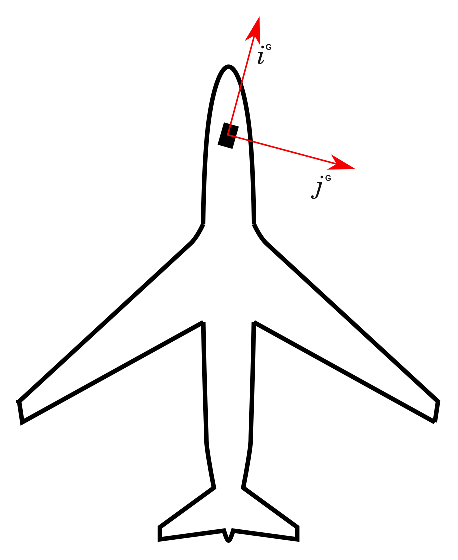
\includegraphics[width=0.3\textwidth]{Contenido/Cuerpo/Capitulo3/Fig7.eps}
	\captionof{figure}{Marco de referencia del la cámara.}
	\label{fig:ModeloMat:Fig1}
\end{center}
De donde el subíndice G hace referencia a que estamos en el plano de la gimbal. El vector unitario K apunta hacia afuera,
es decir hacia nosotros.

% --------------------------
% Back matter
% --------------------------
%
{%
\setstretch{1.1}
\renewcommand{\bibfont}{\normalfont\small}
\setlength{\biblabelsep}{0pt}
\setlength{\bibitemsep}{0.5\baselineskip plus 0.5\baselineskip}
\printbibliography[nottype=online]
\newrefcontext[labelprefix={@}]
\printbibliography[heading=subbibliography,title={Webpages},type=online]
}

\cleardoublepage

\listoffigures
\cleardoublepage

\listoftables
\cleardoublepage

% \lstlistoflistings
% \cleardoublepage

% \appendix\cleardoublepage
% \input{content/chapter-appendix}       % INCLUDE: appendix

% \cleardoublepage
% \input{content/colophon}

% \cleardoublepage
% \input{content/declaration}
% \clearpage

\newpage
\mbox{}


% **************************************************
% End of Document CONTENT
% **************************************************
\end{document}

